%%
%% This is file `sample-manuscript.tex',
%% generated with the docstrip utility.
%%
%% The original source files were:
%%
%% samples.dtx  (with options: `manuscript')
%% 
%% IMPORTANT NOTICE:
%% 
%% For the copyright see the source file.
%% 
%% Any modified versions of this file must be renamed
%% with new filenames distinct from sample-manuscript.tex.
%% 
%% For distribution of the original source see the terms
%% for copying and modification in the file samples.dtx.
%% 
%% This generated file may be distributed as long as the
%% original source files, as listed above, are part of the
%% same distribution. (The sources need not necessarily be
%% in the same archive or directory.)
%%
%% Commands for TeXCount
%TC:macro \cite [option:text,text]
%TC:macro \citep [option:text,text]
%TC:macro \citet [option:text,text]
%TC:envir table 0 1
%TC:envir table* 0 1
%TC:envir tabular [ignore] word
%TC:envir displaymath 0 word
%TC:envir math 0 word
%TC:envir comment 0 0
%%
%%
%% The first command in your LaTeX source must be the \documentclass command.
%%%% Small single column format, used for CIE, CSUR, DTRAP, JACM, JDIQ, JEA, JERIC, JETC, PACMCGIT, TAAS, TACCESS, TACO, TALG, TALLIP (formerly TALIP), TCPS, TDSCI, TEAC, TECS, TELO, THRI, TIIS, TIOT, TISSEC, TIST, TKDD, TMIS, TOCE, TOCHI, TOCL, TOCS, TOCT, TODAES, TODS, TOIS, TOIT, TOMACS, TOMM (formerly TOMCCAP), TOMPECS, TOMS, TOPC, TOPLAS, TOPS, TOS, TOSEM, TOSN, TQC, TRETS, TSAS, TSC, TSLP, TWEB.
% \documentclass[acmsmall]{acmart}

%%%% Large single column format, used for IMWUT, JOCCH, PACMPL, POMACS, TAP, PACMHCI
% \documentclass[acmlarge,screen]{acmart}

%%%% Large double column format, used for TOG
% \documentclass[acmtog, authorversion]{acmart}

%%%% Generic manuscript mode, required for submission
%%%% and peer review
\documentclass[sigchi,screen]{acmart}

%% THIS REMOVES THE ACM THINGS ON THE FIRST PAGE
\settopmatter{printacmref=false}
\renewcommand\footnotetextcopyrightpermission[1]{}
\pagestyle{plain}

%% Fonts used in the template cannot be substituted; margin 
%% adjustments are not allowed.
%%
%% \BibTeX command to typeset BibTeX logo in the docs
\AtBeginDocument{%
  \providecommand\BibTeX{{%
    \normalfont B\kern-0.5em{\scshape i\kern-0.25em b}\kern-0.8em\TeX}}}

%% Rights management information.  This information is sent to you
%% when you complete the rights form.  These commands have SAMPLE
%% values in them; it is your responsibility as an author to replace
%% the commands and values with those provided to you when you
%% complete the rights form.
\setcopyright{acmlicensed}
\copyrightyear{2024}
\acmYear{2024}
\acmDOI{XXXXXXX.XXXXXXX}

%% These commands are for a PROCEEDINGS abstract or paper.
\acmConference[ML4IM]{Machine Learning meets Insect Monitoring - Detecting Tiny Objects in Cluttered Natural Outdoor Environments }{October 2023 -- March 2024}{M\"unster, Germany}
%
%  Uncomment \acmBooktitle if th title of the proceedings is different
%  from ``Proceedings of ...''!
%
%\acmBooktitle{Woodstock '18: ACM Symposium on Neural Gaze Detection,
% June 03--05, 2018, Woodstock, NY} 
%\acmISBN{978-1-4503-XXXX-X/18/06}


%%
%% Submission ID.
%% Use this when submitting an article to a sponsored event. You'll
%% receive a unique submission ID from the organizers
%% of the event, and this ID should be used as the parameter to this command.
%%\acmSubmissionID{123-A56-BU3}

%%
%% For managing citations, it is recommended to use bibliography
%% files in BibTeX format.
%%
%% You can then either use BibTeX with the ACM-Reference-Format style,
%% or BibLaTeX with the acmnumeric or acmauthoryear sytles, that include
%% support for advanced citation of software artefact from the
%% biblatex-software package, also separately available on CTAN.
%%
%% Look at the sample-*-biblatex.tex files for templates showcasing
%% the biblatex styles.
%%

%%
%% The majority of ACM publications use numbered citations and
%% references.  The command \citestyle{authoryear} switches to the
%% "author year" style.
%%
%% If you are preparing content for an event
%% sponsored by ACM SIGGRAPH, you must use the "author year" style of
%% citations and references.
%% Uncommenting
%% the next command will enable that style.
%%\citestyle{acmauthoryear}
\usepackage{multicol}
\usepackage{tikz}
\usetikzlibrary{shapes, arrows, positioning,arrows.meta,calc}
\usepackage{xcolor}
\usepackage{pgfplots}
\pgfplotsset{width=\linewidth,compat=1.9}
\usepackage{subcaption} % for subfigures
\usepackage{todonotes}
\usepackage{multirow}
\usepackage{csvsimple}
\usepackage{longtable}
\usepackage{xstring}
\usepackage[T1]{fontenc}
\usepackage{stringstrings}

%%
%% end of the preamble, start of the body of the document source.
\begin{document}

%%
%% The "title" command has an optional parameter,
%% allowing the author to define a "short title" to be used in page headers.
\title{Machine Learning meets Insect Monitoring}

%%
%% The "author" command and its associated commands are used to define
%% the authors and their affiliations.
%% Of note is the shared affiliation of the first two authors, and the
%% "authornote" and "authornotemark" commands
%% used to denote shared contribution to the research.
\author{Jakob Danel}
\authornote{Both authors contributed equally to this research.}
\email{jakob.danel@uni-muenster.de}
\affiliation{%
  \institution{Institute for Geoinformatics}
  \streetaddress{Heisenbergstraße 2}
  \city{M\"unster}
  \country{Germany}
  \postcode{48149}
}

\author{Frederick Bruch}
\authornotemark[1]
\email{f_bruc03@uni-muenster.de}
\affiliation{%
  \institution{Institute for Geoinformatics}
  \streetaddress{Heisenbergstraße 2}
  \city{M\"unster}
  \country{Germany}
  \postcode{48149}
}

%%
%% By default, the full list of authors will be used in the page
%% headers. Often, this list is too long, and will overlap
%% other information printed in the page headers. This command allows
%% the author to define a more concise list
%% of authors' names for this purpose.
\renewcommand{\shortauthors}{Danel, J. and Bruch, F.}

%%
%% The abstract is a short summary of the work to be presented in the
%% article.
% \begin{abstract}
% \end{abstract}

%%
%% The code below is generated by the tool at http://dl.acm.org/ccs.cfm.
%% Please copy and paste the code instead of the example below.
%%
% \begin{CCSXML}
% <ccs2012>
%  <concept>
%   <concept_id>00000000.0000000.0000000</concept_id>
%   <concept_desc>Do Not Use This Code, Generate the Correct Terms for Your Paper</concept_desc>
%   <concept_significance>500</concept_significance>
%  </concept>
%  <concept>
%   <concept_id>00000000.00000000.00000000</concept_id>
%   <concept_desc>Do Not Use This Code, Generate the Correct Terms for Your Paper</concept_desc>
%   <concept_significance>300</concept_significance>
%  </concept>
%  <concept>
%   <concept_id>00000000.00000000.00000000</concept_id>
%   <concept_desc>Do Not Use This Code, Generate the Correct Terms for Your Paper</concept_desc>
%   <concept_significance>100</concept_significance>
%  </concept>
%  <concept>
%   <concept_id>00000000.00000000.00000000</concept_id>
%   <concept_desc>Do Not Use This Code, Generate the Correct Terms for Your Paper</concept_desc>
%   <concept_significance>100</concept_significance>
%  </concept>
% </ccs2012>
% \end{CCSXML}

% \ccsdesc[500]{Do Not Use This Code~Generate the Correct Terms for Your Paper}
% \ccsdesc[300]{Do Not Use This Code~Generate the Correct Terms for Your Paper}
% \ccsdesc{Do Not Use This Code~Generate the Correct Terms for Your Paper}
% \ccsdesc[100]{Do Not Use This Code~Generate the Correct Terms for Your Paper}

%%
%% Keywords. The author(s) should pick words that accurately describe
%% the work being presented. Separate the keywords with commas.
% \keywords{Do, Not, Us, This, Code, Put, the, Correct, Terms, for,
%   Your, Paper}

%% A "teaser" image appears between the author and affiliation
%% information and the body of the document, and typically spans the
%% page.

%%
%% This command processes the author and affiliation and title
%% information and builds the first part of the formatted document.
\maketitle

% Local IspellDict: en

\section{Introduction}\label{ch01:intro}

The decline of insect populations poses a significant threat to global ecosystems and human livelihoods. As these diminutive creatures play pivotal roles in pollination, nutrient cycling, and pest control, their dwindling numbers could trigger cascading effects throughout food webs, leading to ecosystem instability and agricultural challenges. Amidst growing concerns over insect declines, there is an urgent need for innovative methodologies to monitor and understand insect populations in diverse environments.\\
Our study project, \textit{"Machine Learning meets Insect Monitoring: Detecting Tiny Objects in Cluttered Natural Outdoor Environments"}, addresses this pressing issue by leveraging advanced technologies at the intersection of machine learning and insect ecology. We aim to develop novel approaches for quantifying insect presence in complex outdoor settings.

\subsection{Context and Motivation}

The motivation for our project stems from the alarming decline in insect populations and its potential catastrophic consequences for ecosystems and human society. Quantitative data paints a dire picture, indicating that 41\% of global insect species have declined over the past century alone \citep{sanchez2019worldwide}. This decline is not limited to terrestrial insects but also affects non-terrestrial species. Furthermore, while vertebrate populations have garnered significant attention, it's crucial to recognize that more than 90\% of all animal species are invertebrates, with insects making a big part of it. Insects are indispensable for ecosystem health, with 90\% of flowering plants benefiting from their pollination efforts \citep{ollerton2011many}. Their contribution extends to global agriculture, where insect pollinators promote the production of 75\% of major crops, valued at approximately €150 billion \citep{gallai2009economic, eilers2011contribution}. However, monitoring and quantifying invertebrates pose significant challenges due to their vast diversity and the complexity of their habitats. Thus, our project aims to address these challenges by developing innovative technological solutions to monitor and quantify insect populations in natural outdoor environments effectively.\\
Traditional methods for monitoring insect populations, such as manual sampling or trap-based surveys, are labor-intensive, time-consuming, and often provide limited spatial and temporal coverage. Moreover, these methods may not adequately capture the dynamic nature of insect behavior in natural environments. To address these challenges, our project seeks to harness the power of emerging technologies, particularly in the realms of computer vision, machine learning, and sensor technology, to revolutionize insect monitoring efforts.

\subsection{Objectives}

The primary objective of our study project is to develop a state-of-the-art visual insect monitoring system capable of detecting and tracking tiny objects in cluttered outdoor environments. By integrating machine learning algorithms with advanced imaging modalities, such as Dynamic Vision Sensors (DVS), we aim to achieve real-time, high-precision insect detection and tracking.\\
Our study project delves into the critical issue of declining insect populations and their profound implications for ecosystems and human welfare. Recognizing the limitations of conventional insect monitoring methods, we emphasize the pressing need for technological advancements to address this challenge. Central to our approach is the development of a Smart Insect Camera Trap, a novel concept that integrates spatial and temporal cues for enhanced insect detection in outdoor environments. We highlight the significance of this innovation in overcoming the complexities of monitoring fast-moving insects amidst cluttered backgrounds. Moreover, we underscore the potential of Dynamic Vision Sensors in capturing rapid insect motion with precision and efficiency. Our project's organizational structure is delineated through distinct phases, including data annotation, algorithm development, and evaluation.

% Local IspellDict: en
\section{Related Work}\label{ch02:manual}
To address the problem of significant quantity of photos that lack useful information (namely, photographs without insects), a substantial amount of energy consumption, and real-time image processing on limited hardware, many methods have been tried.
\citeauthor{naqvi2022camera} showed that scheduled frame capturing outperformed motion-activated imaging \citep{naqvi2022camera}.
\citeauthor{ratnayake2021towards} used kNN background subtraction and YOLOv2 to process recordings to detect honeybees \citep{ratnayake2021tracking} and later added flower recognition using YOLOv4 \citep{ratnayake2021towards}.
However, challenges remain in accurately capturing and saving insect imagery due to factors such as small object size, fast insect motion, cluttered scenes, and dynamic backgrounds.
Previous work by \citeauthor{thiele2021towards} has demonstrated progress towards visual insect camera traps.\\
They proposed a methodology that incorporates temporal cues, specifically using the HSV* color space, to improve insect detection accuracy. Their quantitative evaluation of detection networks, including YoloV3, Faster RCNN, and MobileNet, demonstrated promising results in terms of average precision, precision, recall, and computational efficiency \citep{thiele2021towards}.\\
To address the limitations mentioned above, researchers have explored alternative technologies such as Dynamic Vision Sensors (DVS). DVS offers several advantages over conventional RGB cameras, as it is specifically designed to detect motion events with high sensitivity, ultra-fast response times, and low energy consumption \citep{delbruck2016neuromorophic}. The utilization of DVS technology holds promise for enhancing insect tracking capabilities within the Smart Insect Camera Trap. 
Building upon this foundation, \citeauthor{Gebauer_2024_WACV} extend the capabilities of insect camera traps by introducing DVS-based sensing in combination with a real-time small object detection algorithm, demonstrating superior detection performance and lower processing times compared to state-of-the-art deep learning models \citep{Gebauer_2024_WACV}.

\section{Fundamentals}

\subsection{Object Detection Measurements}

Confusion matrices (Table \ref{tab:confusion_matrix}) are frequently employed in object detection tasks to assess the effectiveness of our model. This matrix facilitates the evaluation of our model's performance in accurately identifying true positives (correctly detected instances), false positives (incorrectly detected instances), true negatives (correctly rejected instances), and false negatives (missed detections).

\begin{table}[htbp]
  \centering
  \begin{tabular}{@{}cccc@{}}
    & \multicolumn{2}{c}{\textbf{Predicted}} \\ \cmidrule(l){2-3} 
    \textbf{Actual} & \textbf{Positive} & \textbf{Negative} \\ \midrule
    \textbf{Positive} & TP & FP \\
    \textbf{Negative} & FN & TN \\ \bottomrule
  \end{tabular}
  \caption{Confusion matrix explaining true positives (TP), false positives (FP), false negatives (FN), and true negatives (TN).}
  \label{tab:confusion_matrix}
\end{table}
From this matrix, we derive important metrics like \textit{Precision} ($\frac{TP}{TP +FP}$) and \textit{Recall} ($\frac{TP}{TP +FN}$) \citep{aghdam2017guide}, valuing all detections with confidence $>0.25$ and $IoU > 0.45$ as $TP$, where confidence represents the model's confidence in the detection and \textit{IoU} is defined for calculated bounding box $B_p$ and expected bounding box $B_e$ as: $\frac{B_p \cup B_e}{B_p \cap B_e} = \frac{\text{area of overlap}}{\text{area of union}}$ \citep{szeliski2022computer}. \\
\textit{Mean Average Precision} (mAP) is calculated as the area under the Precision-Recall Curve \citep{everingham2010pascal}. The Precision-Recall Curve is calculated by examining all confidence thresholds and calculating Precision and Recall. \\
Additionally, we introduce the concept of fitness to assess the model's performance comprehensively. The fitness metric is defined as the best fitness over all epochs and is calculated as follows:
\[ \text{fitness} = 0.1 \times \text{mAP@0.5} + 0.9 \times \text{mAP@0.5-0.95} \] Here, mAP@0.5 represents the mean average precision at an IoU threshold of 0.5, while mAP@0.5-0.95 represents the mean average precision across IoU thresholds ranging from 0.5 to 0.95. This composite metric provides a balanced assessment of the model's performance across different IoU thresholds, with greater emphasis placed on higher IoU thresholds to ensure robustness in object detection.

\subsection{Hardware and Camera Setup}
\label{ch:hardware-setup}
The insect monitoring system (see Figure \ref{fig:dvs-system}) relies on a carefully designed hardware setup comprising two key components: a conventional full-frame RGB camera and a Dynamic Vision Sensor (DVS).

\subsubsection{RGB Camera}
The RGB camera, a Basler a2A1920-160ucBAS with a resolution of 2.3 MP and a frame rate of 160 fps, is equipped with a Kowa LM16JC1MS 16mm/F1.4 C-Mount lens. This high-resolution RGB camera captures visual data at a rapid frame rate of 160 fps, providing detailed imagery of the monitored environment.

\subsubsection{Dynamic Vision Sensor}
The DVS operates on neuromorphic vision principles, detecting events triggered by local brightness changes above a threshold. It offers high-temporal-resolution event data suitable for tracking fast-moving insects in cluttered and dynamic environments. The DVS used is a Prophesee EVK4 connected with a Trigger Connector.

\subsubsection{Beamsplitter}
The RGB camera and the DVS are positioned in front of the same beamsplitter, with 70\% of the light reserved for the RGB camera and 30\% for the DVS. Both cameras are housed in a 3D-printed enclosure to ensure they have a similar view of the captured scene. Both cameras use a Kowa LM16JC1MS 16mm/F1.4 C-Mount lens, and the focus is set to a plant about one meter away from the camera.

% This hardware configuration forms the foundation of our insect monitoring system, enabling comprehensive and real-time monitoring of insect populations in natural outdoor environments. By leveraging the complementary advantages of traditional visual data and event-based data, our system offers a holistic approach to insect monitoring, paving the way for enhanced insights into insect behavior and ecosystem dynamics.

\begin{figure}[htbp] % You can specify the position of the figure (h: here, t: top, b: bottom, p: page)
    \centering % Center the image
    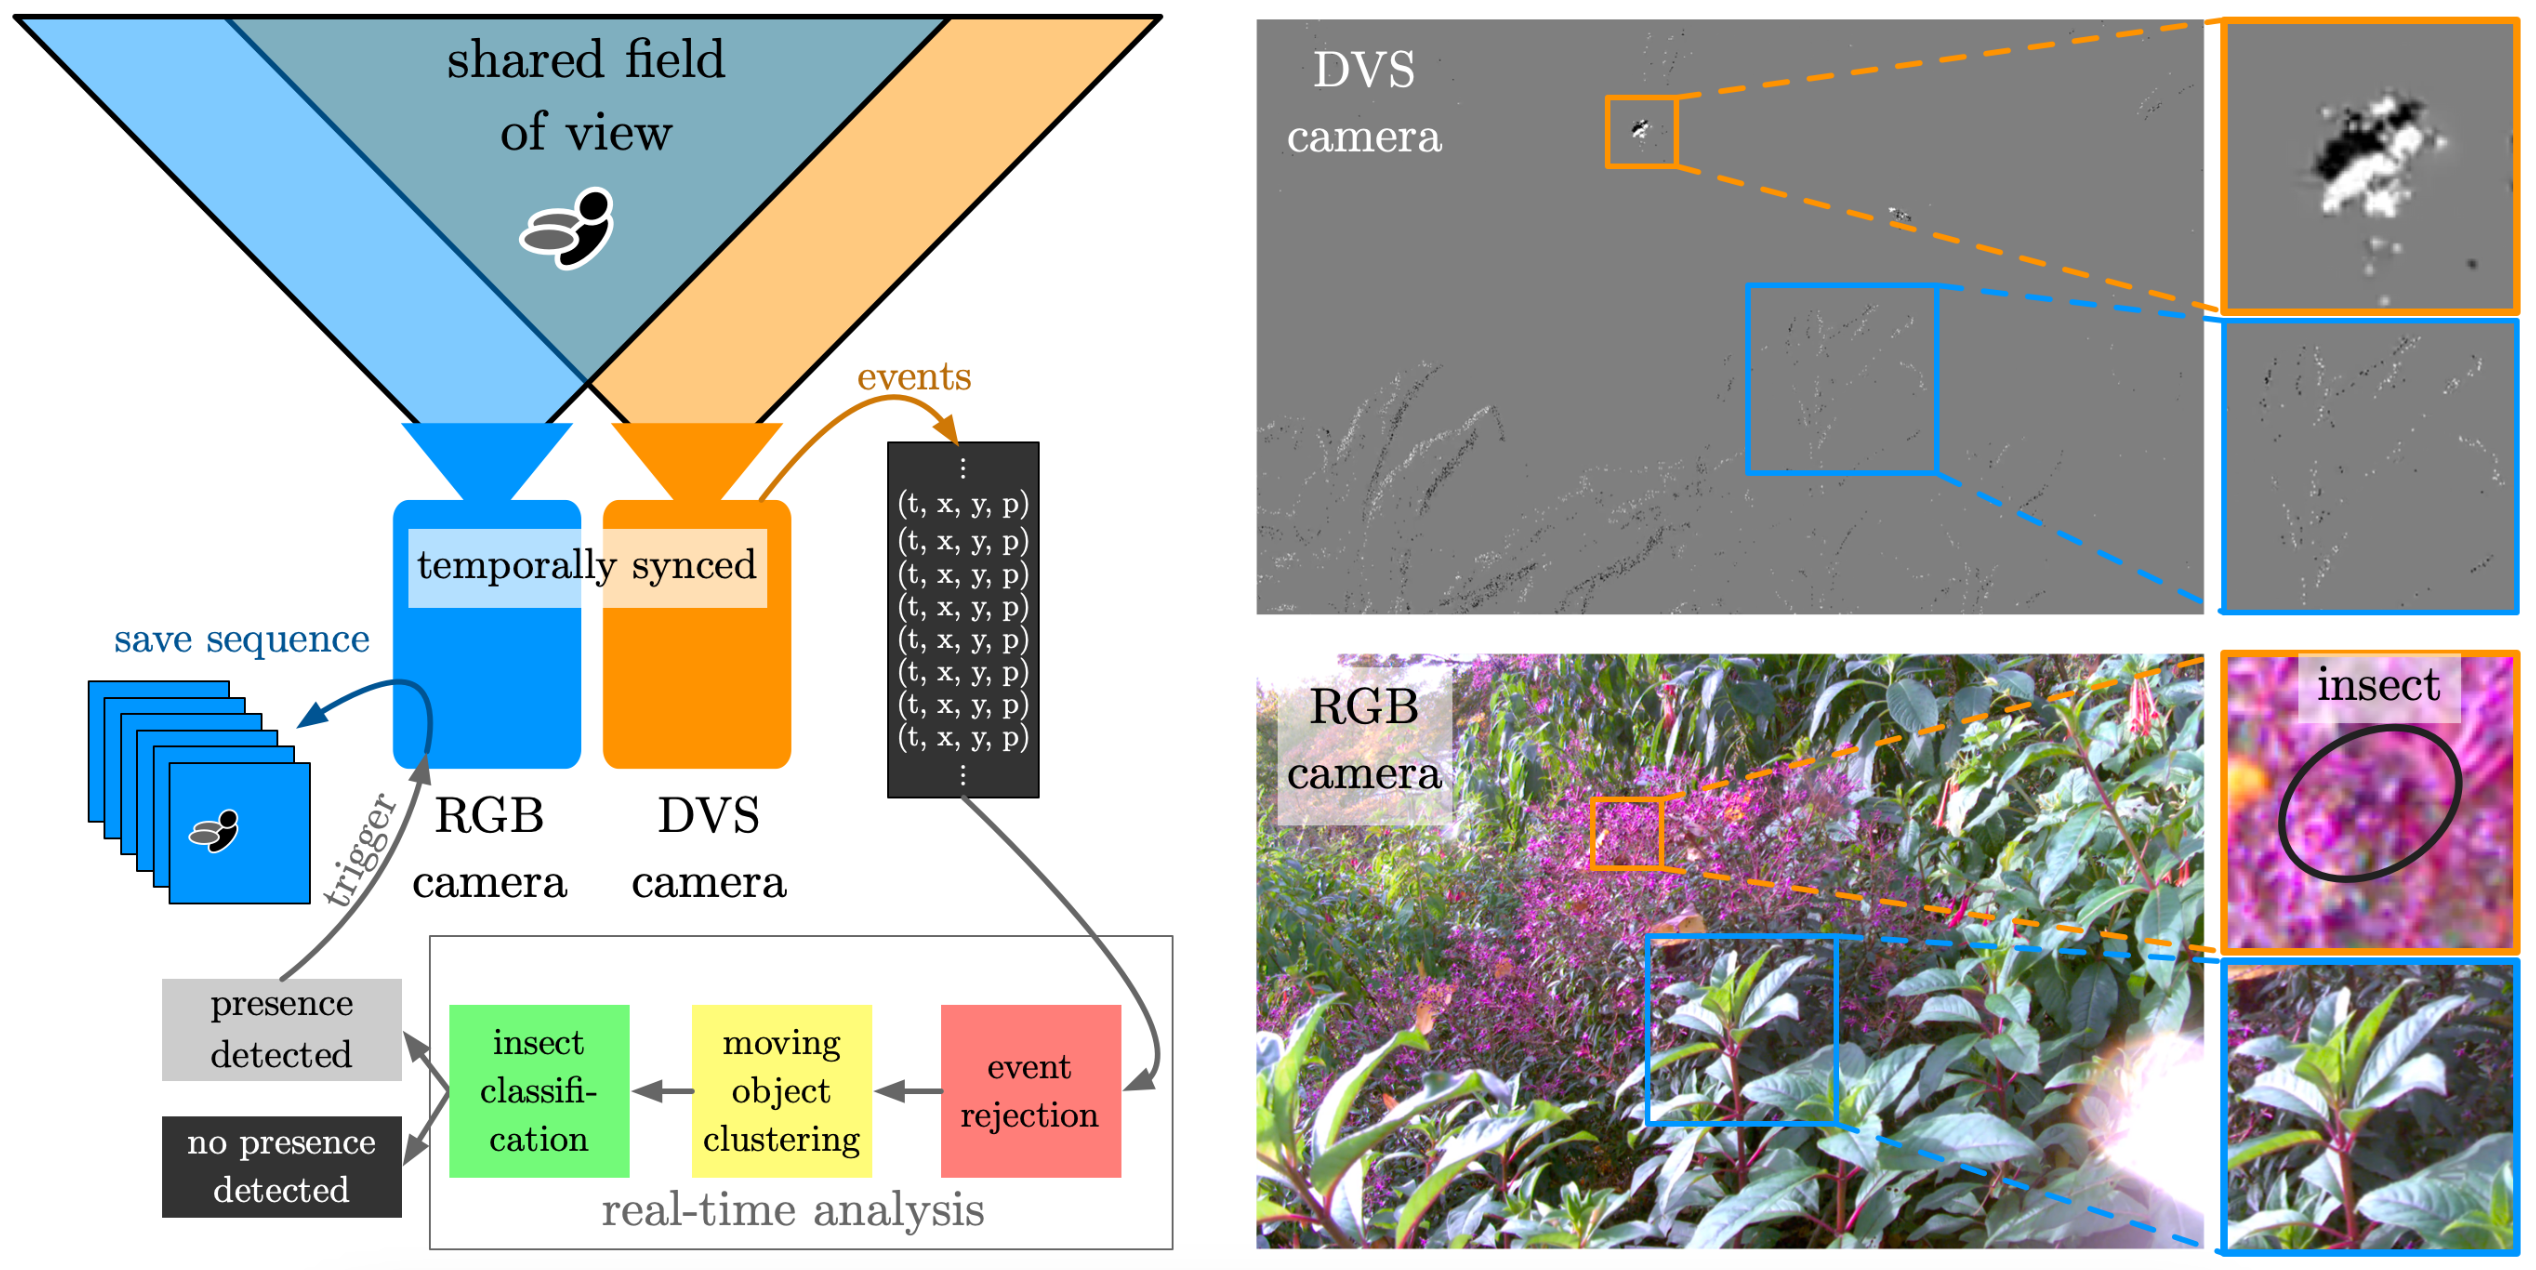
\includegraphics[width=\linewidth]{figures/dvs-system.png} % Change 'example-image' to the filename of your image
    \caption{RGB-DVS Camera System \cite{Gebauer_2024_WACV}.} % Caption for the image
    \label{fig:dvs-system} % A label to refer to the figure in the text
\end{figure}

\subsection{CNN's and YOLO}

The first precursor of a convolutional neural network (CNN), named Neocognitron, was published in 1990. It established the ideas of feature extraction, pooling layers, and convolution in a neural network \cite{fukushima1980neocognitron}. The term "convolutional neural network" was coined to describe the architecture of the LeNet\cite{lecun1998gradient}, which was developed by Yann LeCun and his team from 1989 to 1998 for the handwritten digit recognition task. With AlexNet\cite{krizhevsky2012imagenet}, the first ever CNN won the ImageNet\footnote{\url{https://image-net.org/index.php}} classification challenge in 2012, reducing the error rate from  26.2\% to 15.3\%. Since then, every winner of the ‘ImageNet large scale visual recognition challenge (ILSVRC)’ was based on a CNN.\\
In 2016, a new convolutional neural network (CNN) named YOLO (You Only Look Once) was released by Joseph Redmon and his team \cite{Redmon_2016_CVPR}. This revolutionary model (see Figure \ref{fig:architecture}) was one of the first models utilizing single-stage method for object detection, surpassing previous detectors in both speed and accuracy. Its remarkable performance quickly established YOLO as one of the most favored architectures for object detection tasks across academic and non-academic circles \cite{scharf2023TEMP}. Since then, numerous researchers and groups have iteratively refined YOLO, with the most recent major version being YOLOv9\cite{wang2024yolov9}.

\begin{figure}[ht] % You can specify the position of the figure (h: here, t: top, b: bottom, p: page)
    \centering % Center the image
    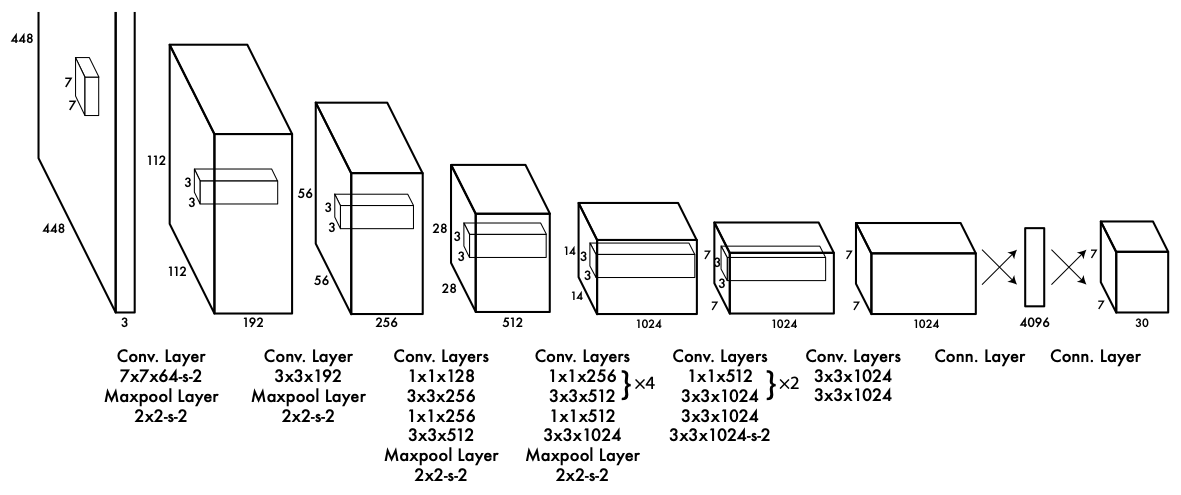
\includegraphics[width=\linewidth]{figures/architecture.png} % Change 'example-image' to the filename of your image
    \caption{YOLO Architecture.} % Caption for the image
    \label{fig:architecture} % A label to refer to the figure in the text
\end{figure}

\subsection{Preprocessing}

Since we will be manipulating the original video streams obtained from the RGB and DVS camera, we will now discuss some fundamental preprocessing techniques.

\subsubsection{Background Subtraction}
Background subtraction is aimed at isolating foreground objects from the background in an image or video stream. The process involves extracting the regions of interest by identifying and removing the stationary elements or the background from the input data. In this study, we utilized the MOG2 (Mixture of Gaussians) background subtraction algorithm from the OpenCV library\footnote{\url{https://pypi.org/project/opencv-python/}}. MOG2 is a robust and widely-used method for background modeling, capable of adaptively updating the background model over time to accommodate gradual illumination changes and dynamic backgrounds.

\subsubsection{Temporal Filter}

Temporal filtering is used in signal and image processing to reduce noise and smooth out fluctuations over time. The basic principle behind temporal filtering involves analyzing the variations in intensity or pixel values across consecutive frames in a video sequence. By considering the temporal relationship between adjacent frames, temporal filters aim to suppress random noise while preserving the underlying structure and motion in the data. One common approach to temporal filtering is the use of moving average or low-pass filters, which compute the average or weighted average of pixel values over a sliding window of frames. In the following experiments, the exponential moving average has been used. This effectively attenuates high-frequency noise components, resulting in a smoother output signal or image sequence. Temporal filtering is particularly useful in scenarios where the input data exhibit temporal instability or jitter, such as in surveillance footage, video streams from mobile cameras, or recordings in noisy environments. 

\subsubsection{RGB to HSV}
\label{ch:pp-hsv}
For transformation from RGB to HSV a classical approach is used, to transform the RGB input stream into the HSV color scheme \cite{CHERNOV2015328}. The HSV values are then written to the RGB-channels of the output. The transformation begins with defining the maximum ($\text{Max} = \max(R, G, B)$) and minimum ($\text{Min} = \min(R, G, B)$) for an input pixel $R, G, B$. Then HSV is defined as following:
\[
\begin{aligned}
    \text{Hue (H)} &= \begin{cases}
            0, & \text{if } \text{Max} = \text{Min} \\
            60^\circ \times \left( \frac{G - B}{\text{Max} - \text{Min}} \mod 6 \right), & \text{if } \text{Max} = R \\
            60^\circ \times \left( \frac{B - R}{\text{Max} - \text{Min}} + 2 \right), & \text{if } \text{Max} = G \\
            60^\circ \times \left( \frac{R - G}{\text{Max} - \text{Min}} + 4 \right), & \text{if } \text{Max} = B
        \end{cases} \\
     \text{Saturation (S)} &= \begin{cases}
        0, & \text{if } \text{Max} = 0 \\
        1 - \frac{\text{Min}}{\text{Max}}, & \text{otherwise}
    \end{cases} \\
    \text{Value (V)} &= \text{Max}
\end{aligned}
\]


\section{Methods}
\tikzset{
  myblock/.style={rectangle, draw, text width=3em, text centered, rounded corners, minimum height=1.5em, font = \tiny},
  ellipsis/.style={
    draw,
    circle,
    inner sep=0,
    minimum size=8pt,
    font = \tiny
  },
  myblock_bigger/.style={rectangle, draw, text width=17em, text centered, rounded corners, minimum height=1.5em, font = \tiny},
  myimage/.style={
    inner sep=0pt,
    outer sep=0pt,
  }
}
\definecolor{col_step1}{RGB}{230,97,1}
\definecolor{col_step2}{RGB}{253,184,99}
\definecolor{col_step3}{RGB}{178,171,210}
\definecolor{col_step4}{RGB}{94,60,153}

\newcommand{\createSplitNode}[4]{
    \node [myblock] at (#1,#2) (#3_#4) {#3: split\_#4};
}
\newcommand{\createTrainConnection}[1]{
    \draw[->](Dataset_#1) --  (Result_#1);
}

\newcommand{\createBDConnection}[1]{
    \draw[->, col_step2](dataset_gt) -- (Dataset_#1);
}

\newcommand{\createdistributionConnection}[1]{
    \draw[->](Result_#1) -- (distribution);
}

\newcommand{\redarrow}{\protect\tikz[baseline=-0.5ex, col_step2]\protect\draw[-{Stealth[col_step2]}, line width=1pt] (0,0) -- (0.5,0);}

\newcommand{\drawNumberedCircleMacro}[3]{%
    \protect\tikz[baseline=(char.base)]{
        \protect\node[circle, draw, fill=#1, inner sep=1pt, outer sep=0pt, text=#3, font=\tiny] (char) {#2};
    }%
}

\begin{figure}[H]
\centering
\begin{tikzpicture}[>=latex, node distance=2.5cm,auto]
  % Define nodes with the myblock style
  \node[myblock] at (1,3.5) (labels_gt) {Labels ground Truth};

  %Commment one out
  % This is for representation as normal box
  %\node[myblock] at (1,5.5) (stacked_imgs) {Stacked Images (Event + RGB)};
  
  %This is for representation as image
  \node[myimage] at (1,5) (stacked_imgs) {\includegraphics[width=3em]{figures/stacked_image_with_frame.png}};

  
  \node [myblock] at (1,2.5) (dataset_gt) {Data Base};
  \createSplitNode{-1}{1}{Dataset}{01}
  \createSplitNode{1}{1}{Dataset}{$i$}
  \createSplitNode{3}{1}{Dataset}{$n$}
  \node [ellipsis] at (0,1) (ellipsisDS1) {...};
  \node [ellipsis] at (2,1) (ellipsisDS2) {...};
  \node [ellipsis] at (0,0) (ellipsisR1) {...};
  \node [ellipsis] at (2,0) (ellipsisR2) {...};

  \createSplitNode{-1}{0}{Result}{01}
  \createSplitNode{1}{0}{Result}{$i$}
  \createSplitNode{3}{0}{Result}{$n$}
  \node [myblock_bigger] at (1,-1) (distribution) {Distribution of metrics (map@0.5, map@0.5--0.95, Precision and Recall)};
  
  
  
  % Draw the upper box (1)
  \draw[dashed, col_step1] ($(stacked_imgs.north west)+(-2.35,0.2)$) rectangle ($(dataset_gt.south east)+(2.2,-0.25)$);
  \node[circle, draw, fill=col_step1, inner sep=1pt, outer sep=0pt, text=white, font=\tiny] at ($(stacked_imgs.north west)+(-2.1,0)$) {\textbf{1}};
  
  % Draw the number for (2)
  \node[circle, draw, fill=col_step2, inner sep=1pt, outer sep=0pt, text=black, font=\tiny] at ($(dataset_gt.south east)+(-3.025,-0.45)$) {\textbf{2}};
  
  % Draw the below box (3)
 \draw[dashed, col_step3] ($(Dataset_01.north west)+(-0.2,0.3)$) rectangle ($(Result_$n$.south east)+(0.2,-0.1)$);
  \node[circle, draw, fill=col_step3, inner sep=1pt, outer sep=0pt, text=black, font=\tiny] at ($(Dataset_01.north west)+(0.15,0.15)$) {\textbf{3}};

  % Drwa the number for (4)
  \node[circle, draw, fill=col_step4, inner sep=1pt, outer sep=0pt, text=white, font=\tiny] at ($(distribution.north west)+(0.4,0.15)$) {\textbf{4}};
  
  
  
  % Define arrows with labels
  \createTrainConnection{01}
  \createTrainConnection{$i$}
  \createTrainConnection{$n$}
  \createBDConnection{01}
  \createBDConnection{$i$}
  \createBDConnection{$n$}
   \createdistributionConnection{01}
   \createdistributionConnection{$i$}
   \createdistributionConnection{$n$}
   \draw[->, col_step2] (dataset_gt) -- (ellipsisDS1);
   \draw[->, col_step2] (dataset_gt) -- (ellipsisDS2);

   \draw[->] (ellipsisDS1) -- (ellipsisR1);
   \draw[->] (ellipsisDS2) -- (ellipsisR2);

 \draw[->] (ellipsisR1) -- (distribution);
 \draw[->] (ellipsisR2) -- (distribution);

 \draw [->] (stacked_imgs.east) to [out=360,in=0] node[right,align=center, font=\tiny]{DVS specific \\ preprocessing} (dataset_gt.east);
  \draw [dashed,->] (stacked_imgs.west) to [out=180,in=180] node[left,align=center, font=\tiny]{(RGB specific \\ preprocessing)} (dataset_gt.west);
 \draw[->] (stacked_imgs) to node[right,align=center, font=\tiny]{Manual\\Labelling} (labels_gt);
 
 \draw[->] (labels_gt) to  (dataset_gt);
\end{tikzpicture}

\caption{Workflow for an experiment with a unique preprocessing combination for DVS (and RGB). Split\_$i$ describing the workflow for one specific scene used for the cross validation (where $i \in\{ i \,|\, i \text{ is an integer, } 1 \leq i \leq n \}$ and $n$ is the amount of scenes in the dataset).}
\label{fig:workflow}
\end{figure}

This section delves into the methods employed throughout our research and provides a rationale for their selection. To clarify essential terms: a "scene" is the setup of the camera within the specific environment, while a "video" consists of smaller segments taken from scenes. Our experimental design encompasses two primary approaches: the DVS only experiment, wherein solely DVS images are used for the detection task, and the RGB + DVS experiment, which involves the utilization of a merged image of both input types for the detection task. To assess the robustness of our experiments, we implemented a cross-validation strategy following the leave-one-out principle. Each scene was designated as validation data for one split, resulting in a distribution of performance quality scores that facilitates meaningful statistical comparisons. A key part of our work involves exploring the impact of different computer vision preprocessings on raw data. Through these experiments, we sought to discern potential enhancements in the detection task performance. The overall workflow of our experiments is visualized in Figure \ref{fig:workflow}, and the subsequent sections will expound upon the applied methods, following the structured framework illustrated in the diagram.


Initially, manual labeling of videos and individual preprocessing procedures are conducted for both RGB and DVS videos,by labeling the DVS stream and mapping the labels to the RGB stream (depicted as \drawNumberedCircleMacro{col_step1}{1}{white}). Then we construct a  dataset that can be used within the YOLO environment for each validation split, with an additional step involving the combination of DVS and RGB data (\drawNumberedCircleMacro{col_step2}{2}{black}). The third step involves employing YOLO for training a model and generating validation results (\drawNumberedCircleMacro{col_step3}{3}{black}). Finally, in the fourth step (\drawNumberedCircleMacro{col_step4}{4}{white}), the study filters the best scores for each validation split and proceeds to compare the distributions of different preprocessing techniques.

\subsection{Preparing the data}
The used dataset was conducted at the Botanical Garden of Mu\"nster. The filming took place from September 28, 2023, to October 13, 2023. The filming process utilized a dual camera setup, as detailed in Section \ref{ch:hardware-setup}. Ten distinct scenes were captured during this period, each scene generating videos comprising a maximum of 4000 frames. In sum, the dataset comprises 97,077 frames. 
% To conduct our experiment, we undertook the preparation of two types of data, focusing on manual labeling for the establishment of a ground truth suitable for training and validation, as well as the implementation of video preprocessing methods aimed at enhancing the model's performance.

\subsubsection{Labelling}
The labeling process was facilitated using the Labelbox tool\footnote{\url{https://labelbox.com/}}. Bounding boxes were drawn around insects identified in each video. Setting bounding boxes for each frame is not required. It is possible to maintain the position of the bounding box unchanged across successive frames.

\subsubsection{Preprocessing}
Video processing was carried out in a stacked format (DVS + RGB), as illustrated in Figure \ref{fig:workflow} at the initial node. This approach provided the advantage of applying the same preprocessing steps to both DVS and RGB data if needed. Given that the DVS input comprises only one-channel information, distinct preprocessing steps were employed on different channels. Furthermore, a sequential preprocessing workflow was implemented. The implementation was done using Python and the framework OpenCV \citep{bradski2000opencv} which is capable of modifying images on pixel base.

\begin{figure}[htp]
  \centering
  \begin{subfigure}{0.25\linewidth}
    \centering
    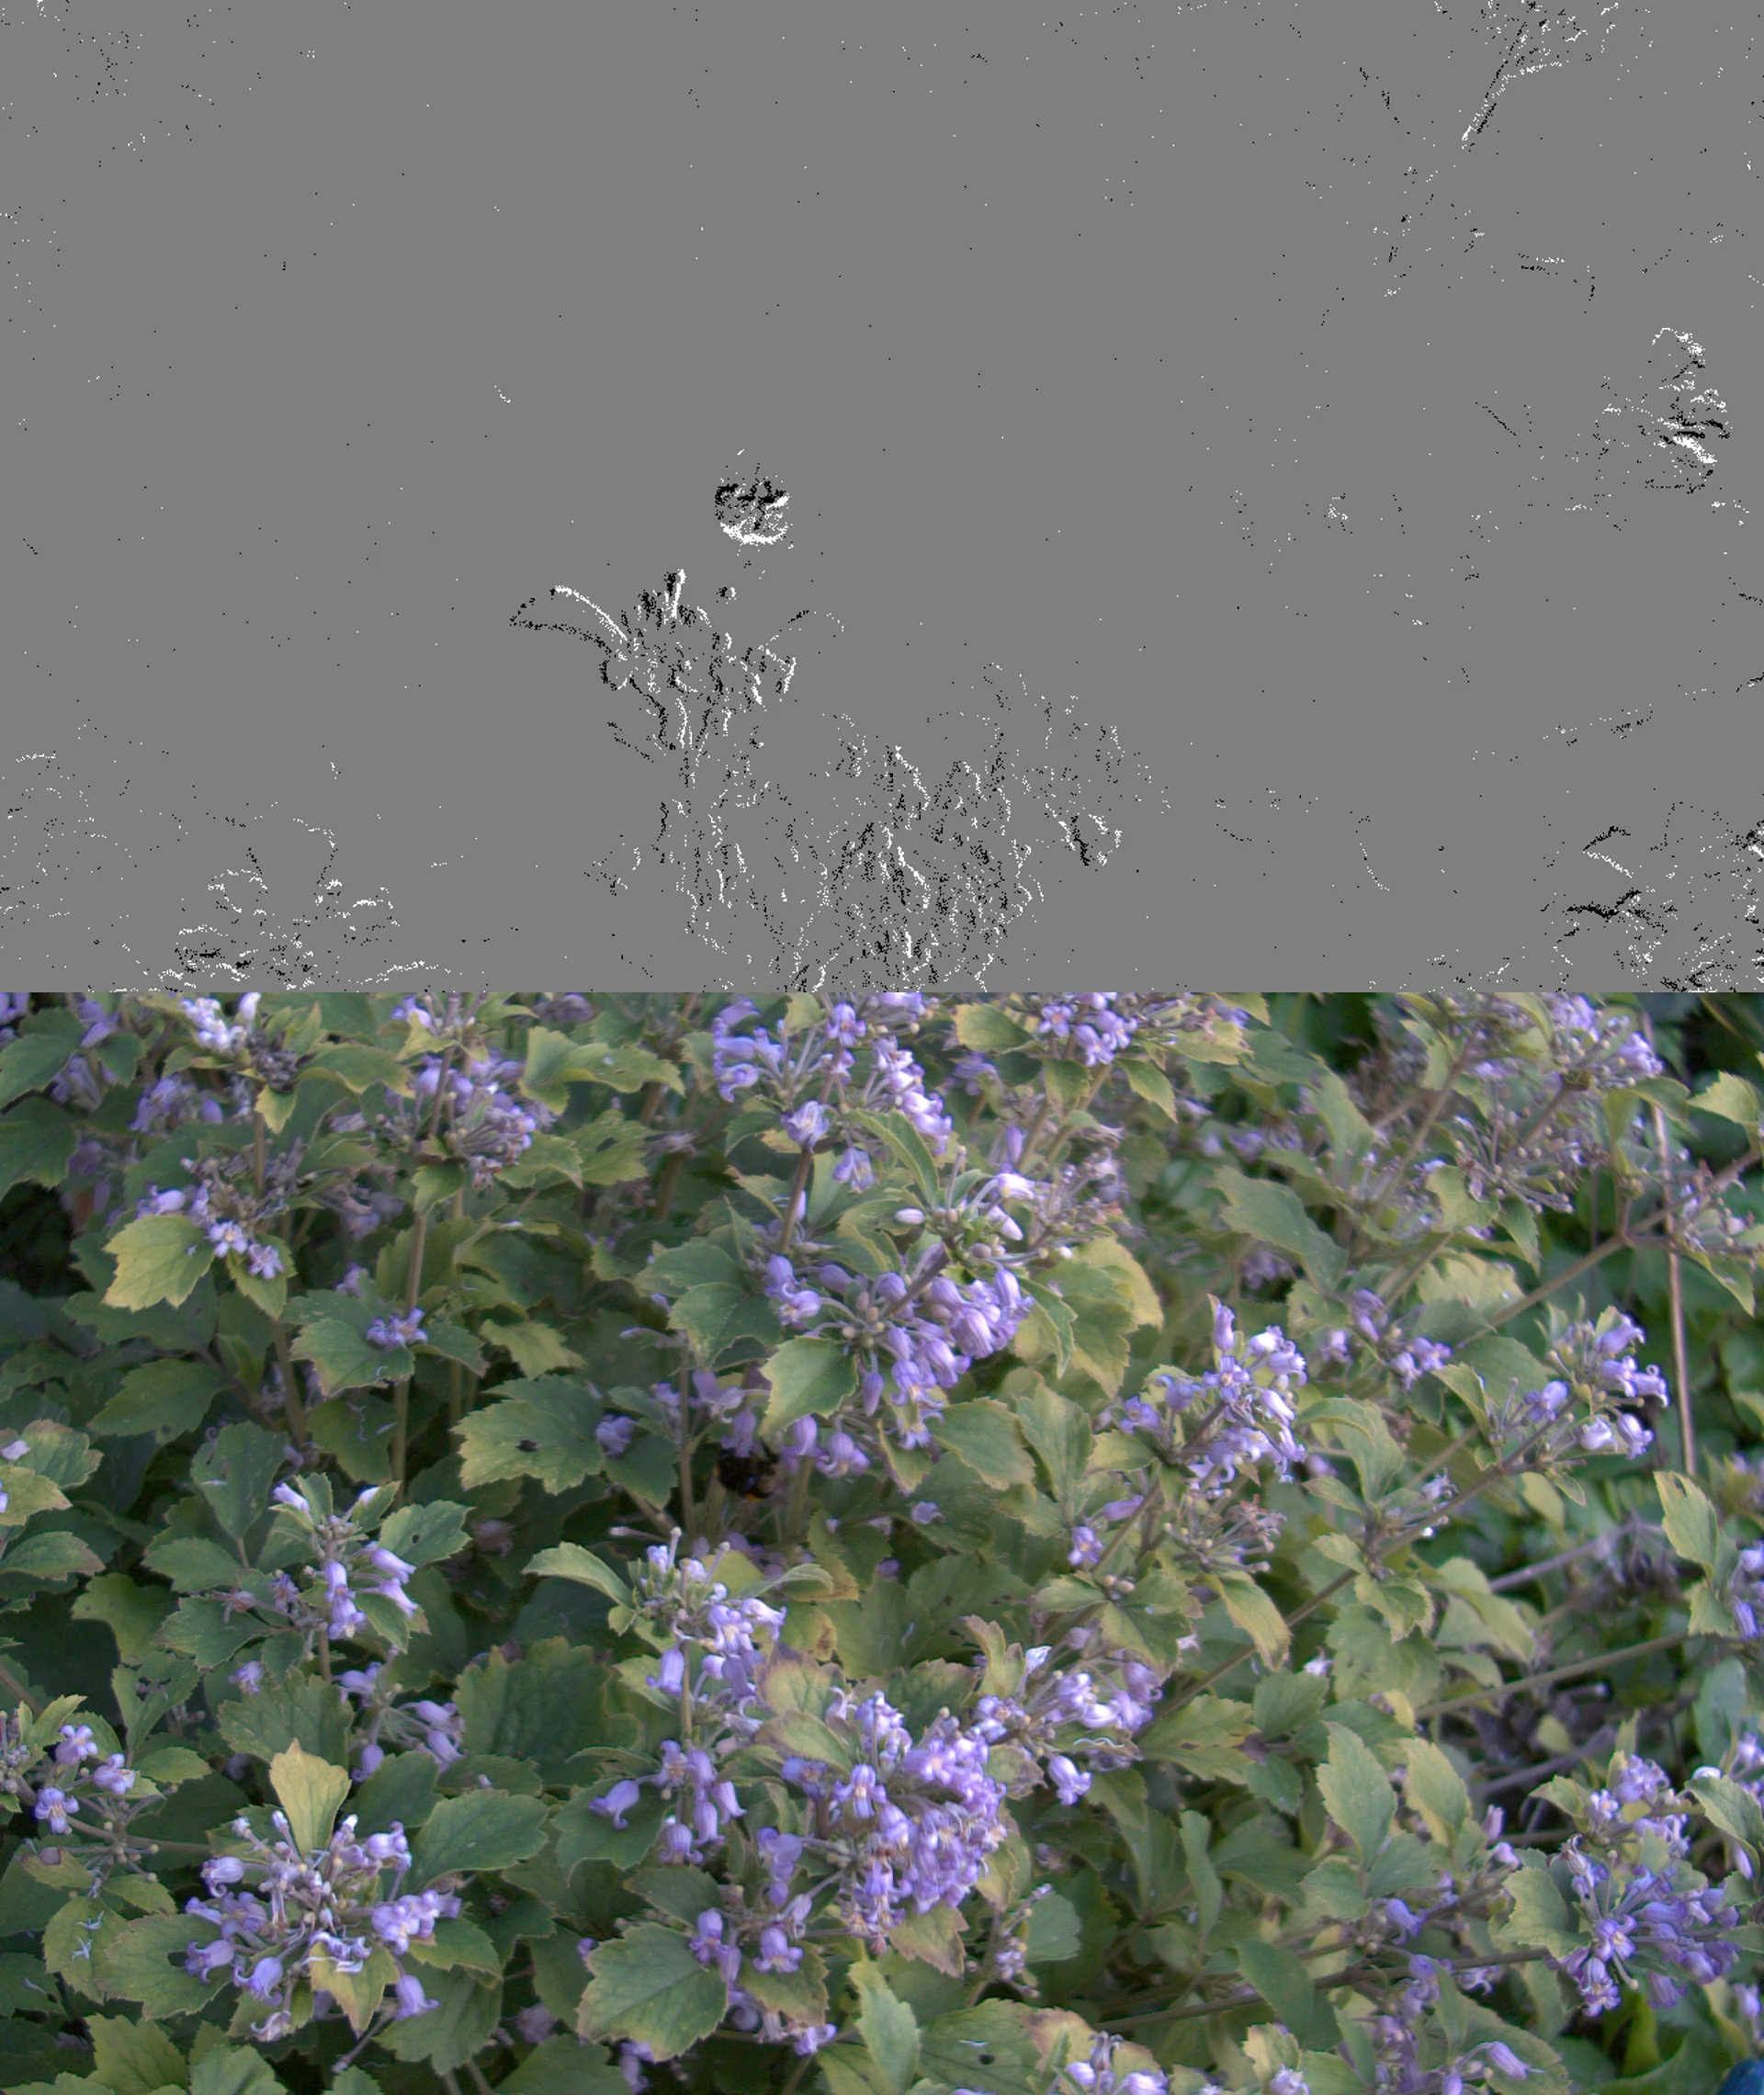
\includegraphics[width=\linewidth]{figures/preprocessings/original.jpg}
    \caption{Original}
  \end{subfigure}%
  \begin{subfigure}{0.25\linewidth}
    \centering
    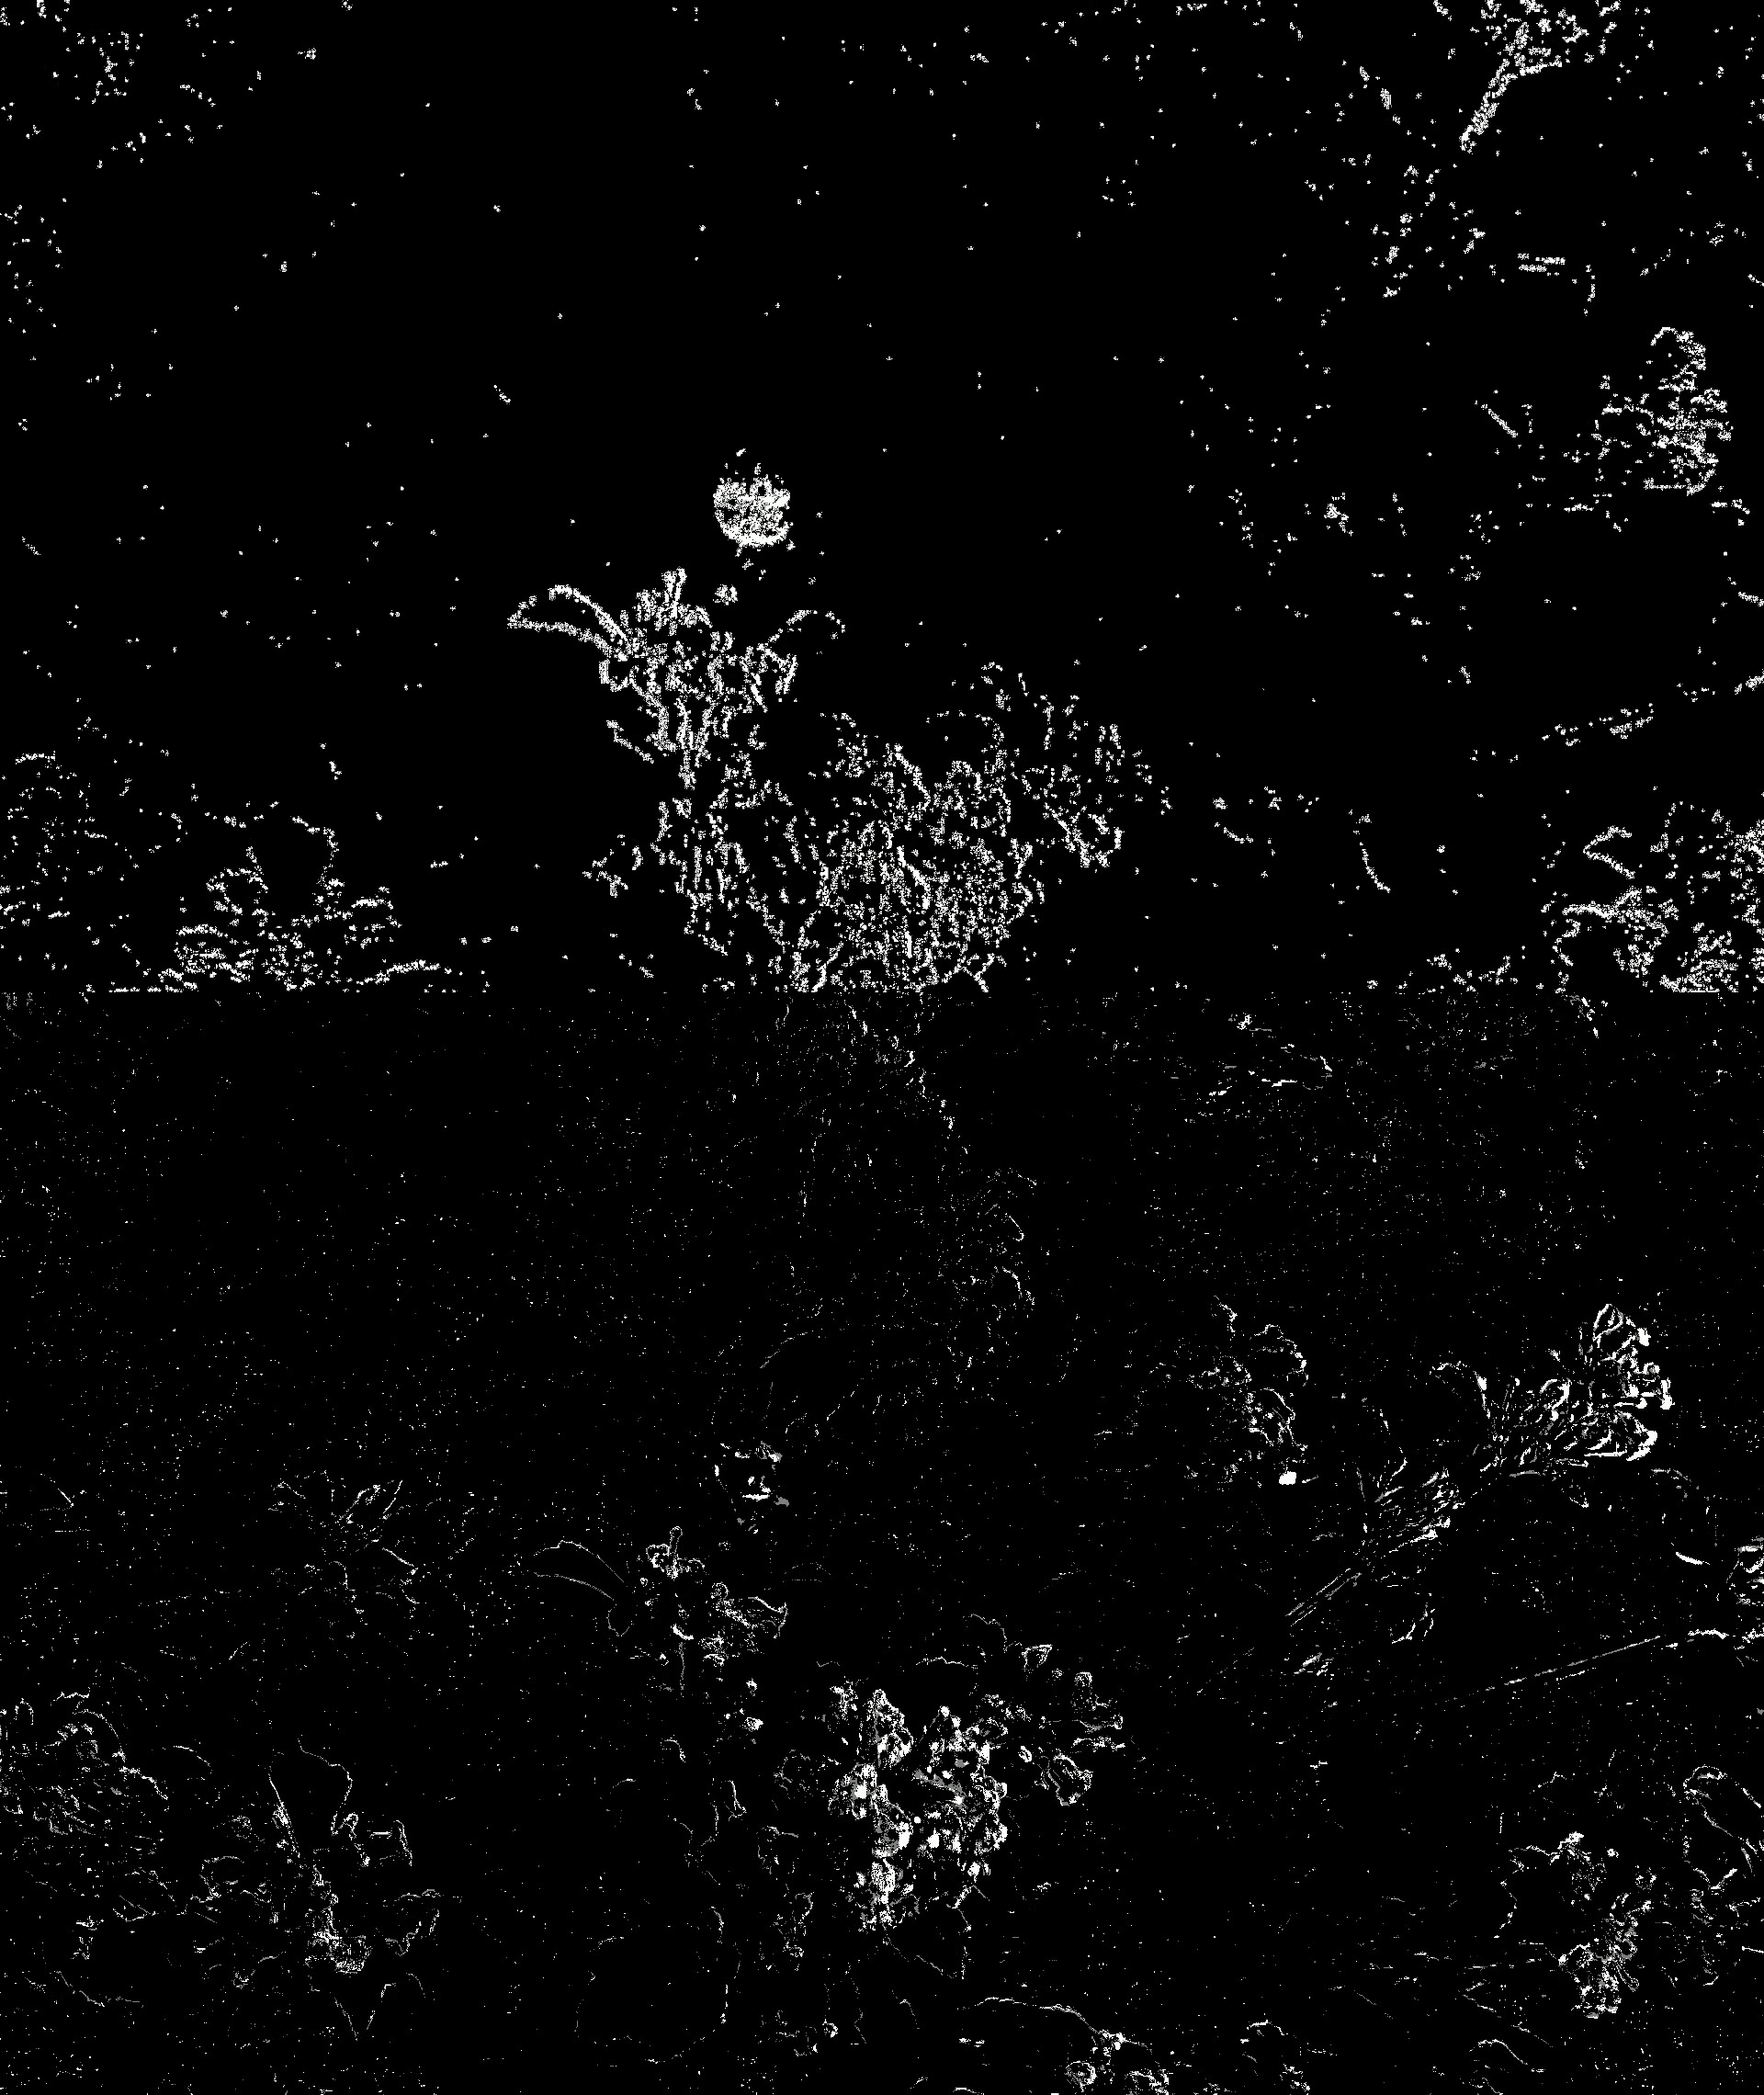
\includegraphics[width=\linewidth]{figures/preprocessings/background_subtraction.jpg}
    \caption{BS}
  \end{subfigure}%
  \begin{subfigure}{0.25\linewidth}
    \centering
    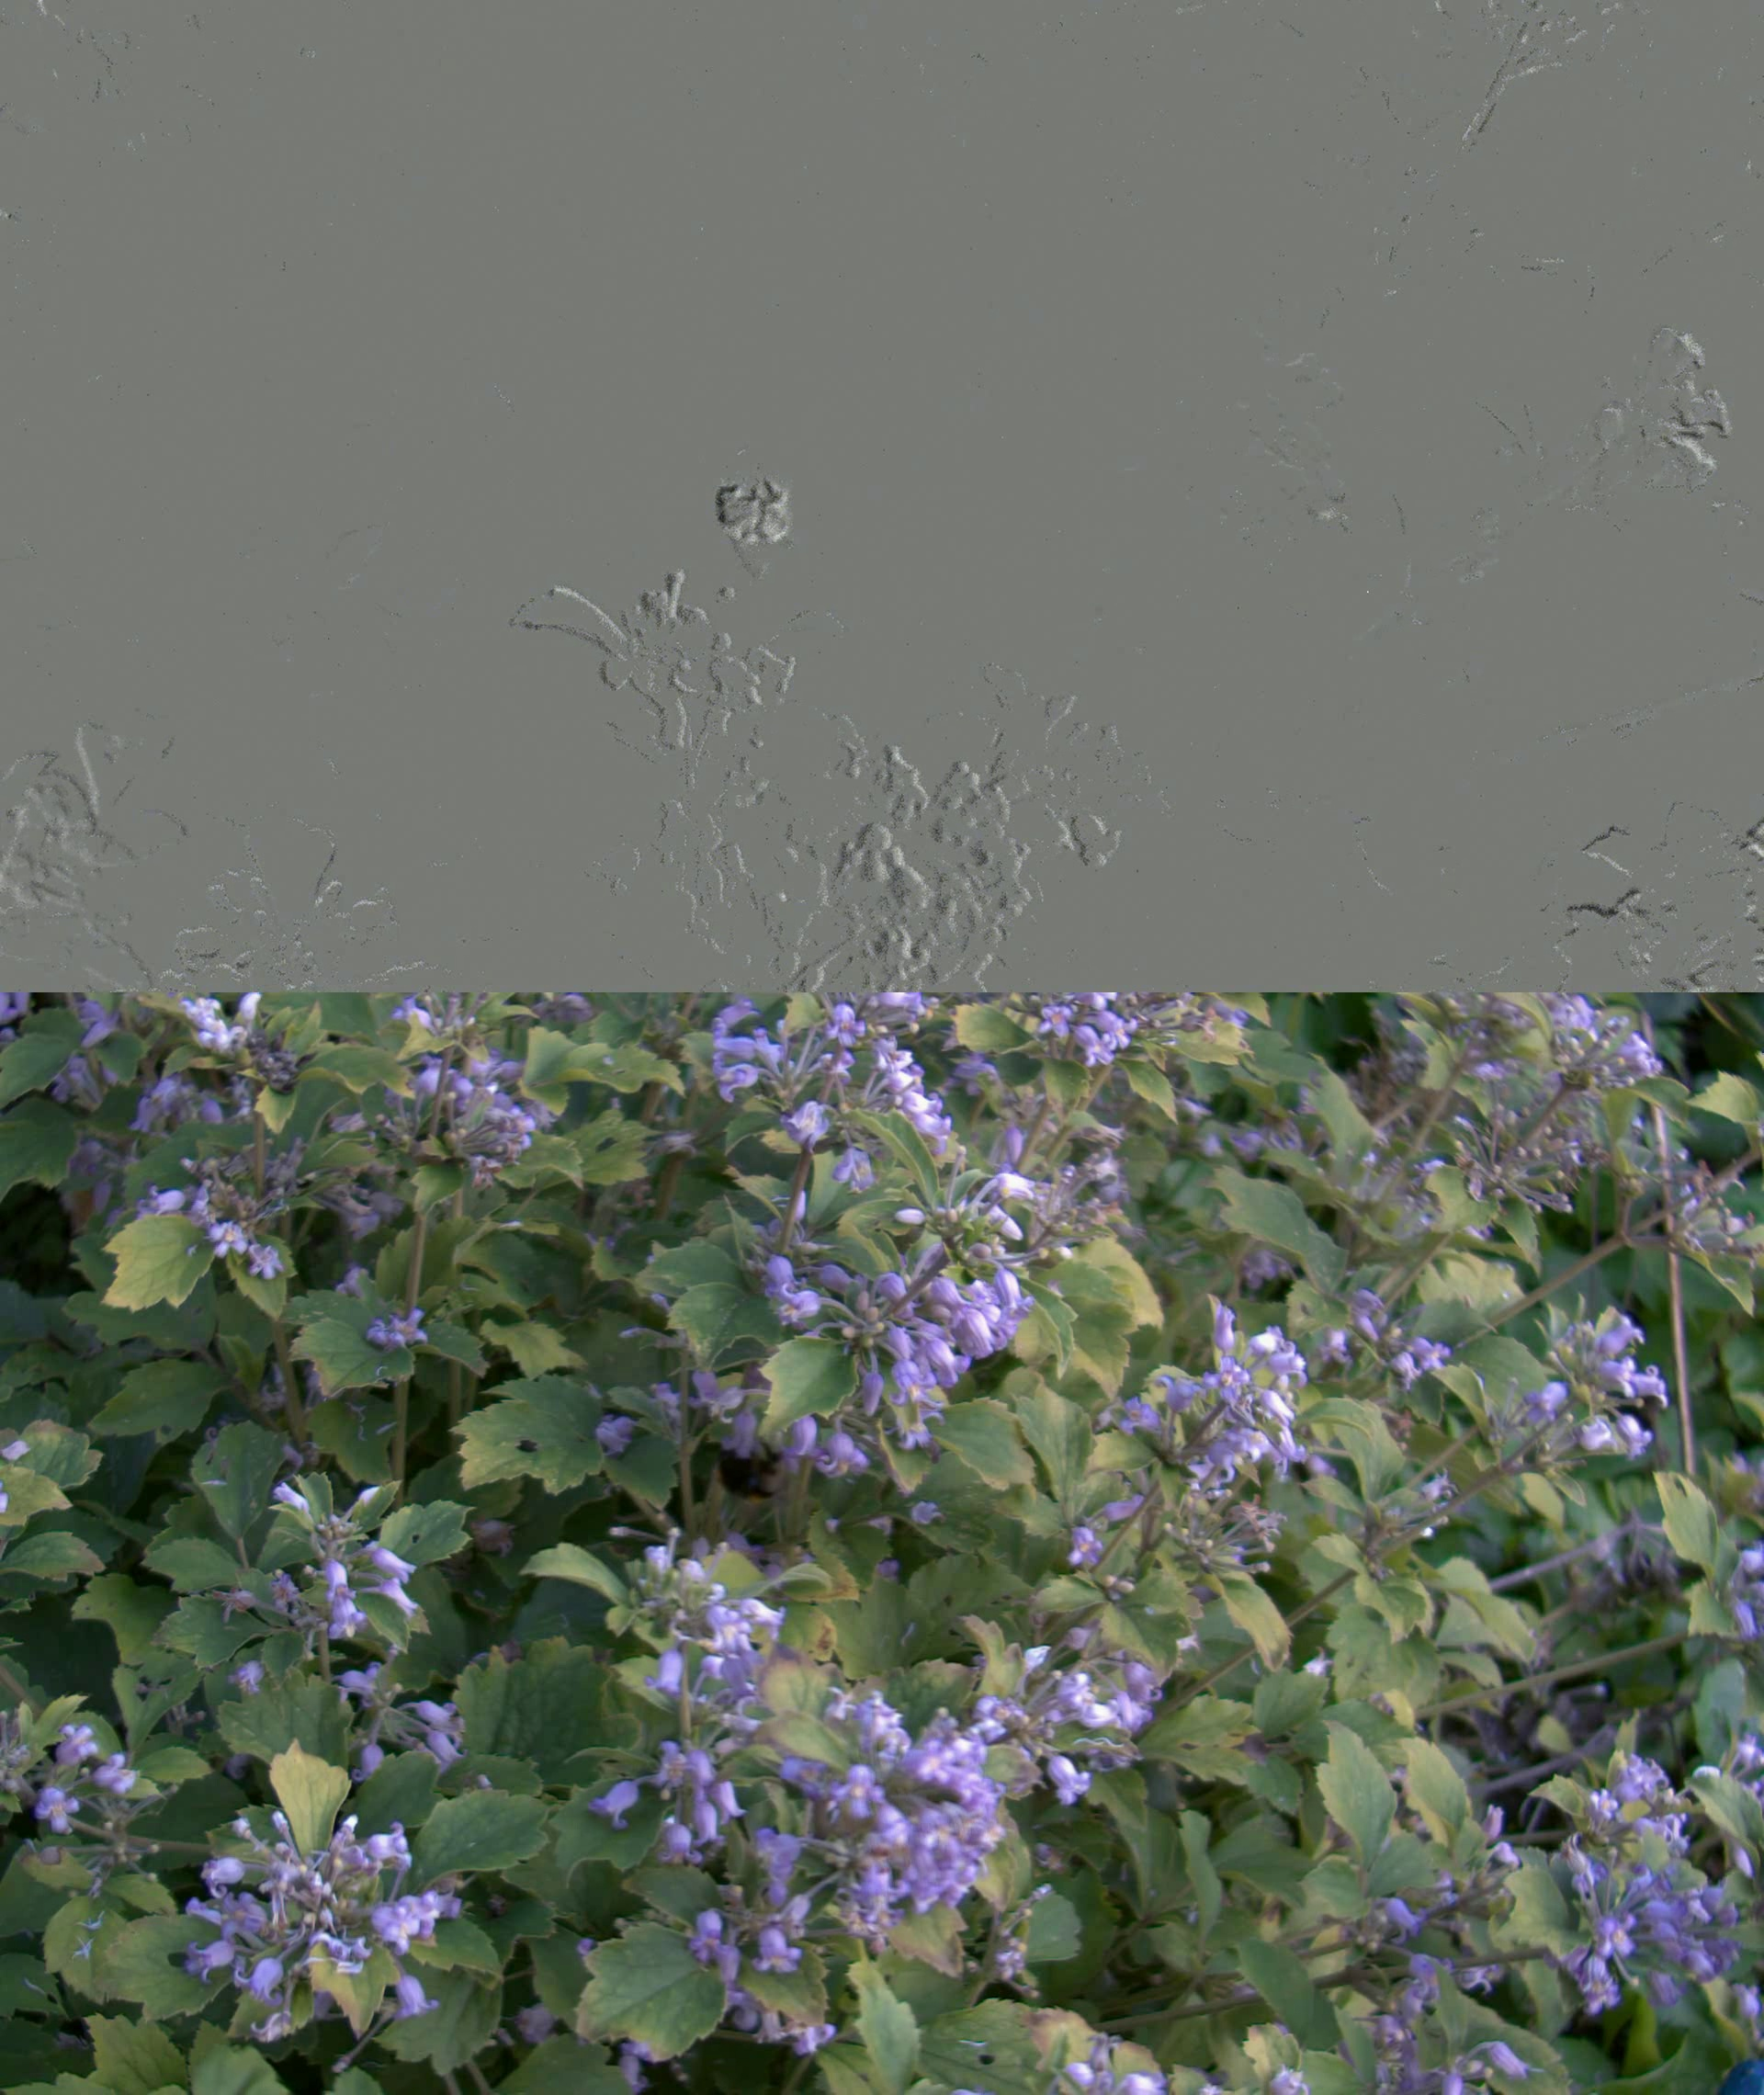
\includegraphics[width=\linewidth]{figures/preprocessings/temporal_filtering.jpg}
    \caption{TF ($fs = 5$)}
  \end{subfigure}%
  \begin{subfigure}{0.25\linewidth}
    \centering
    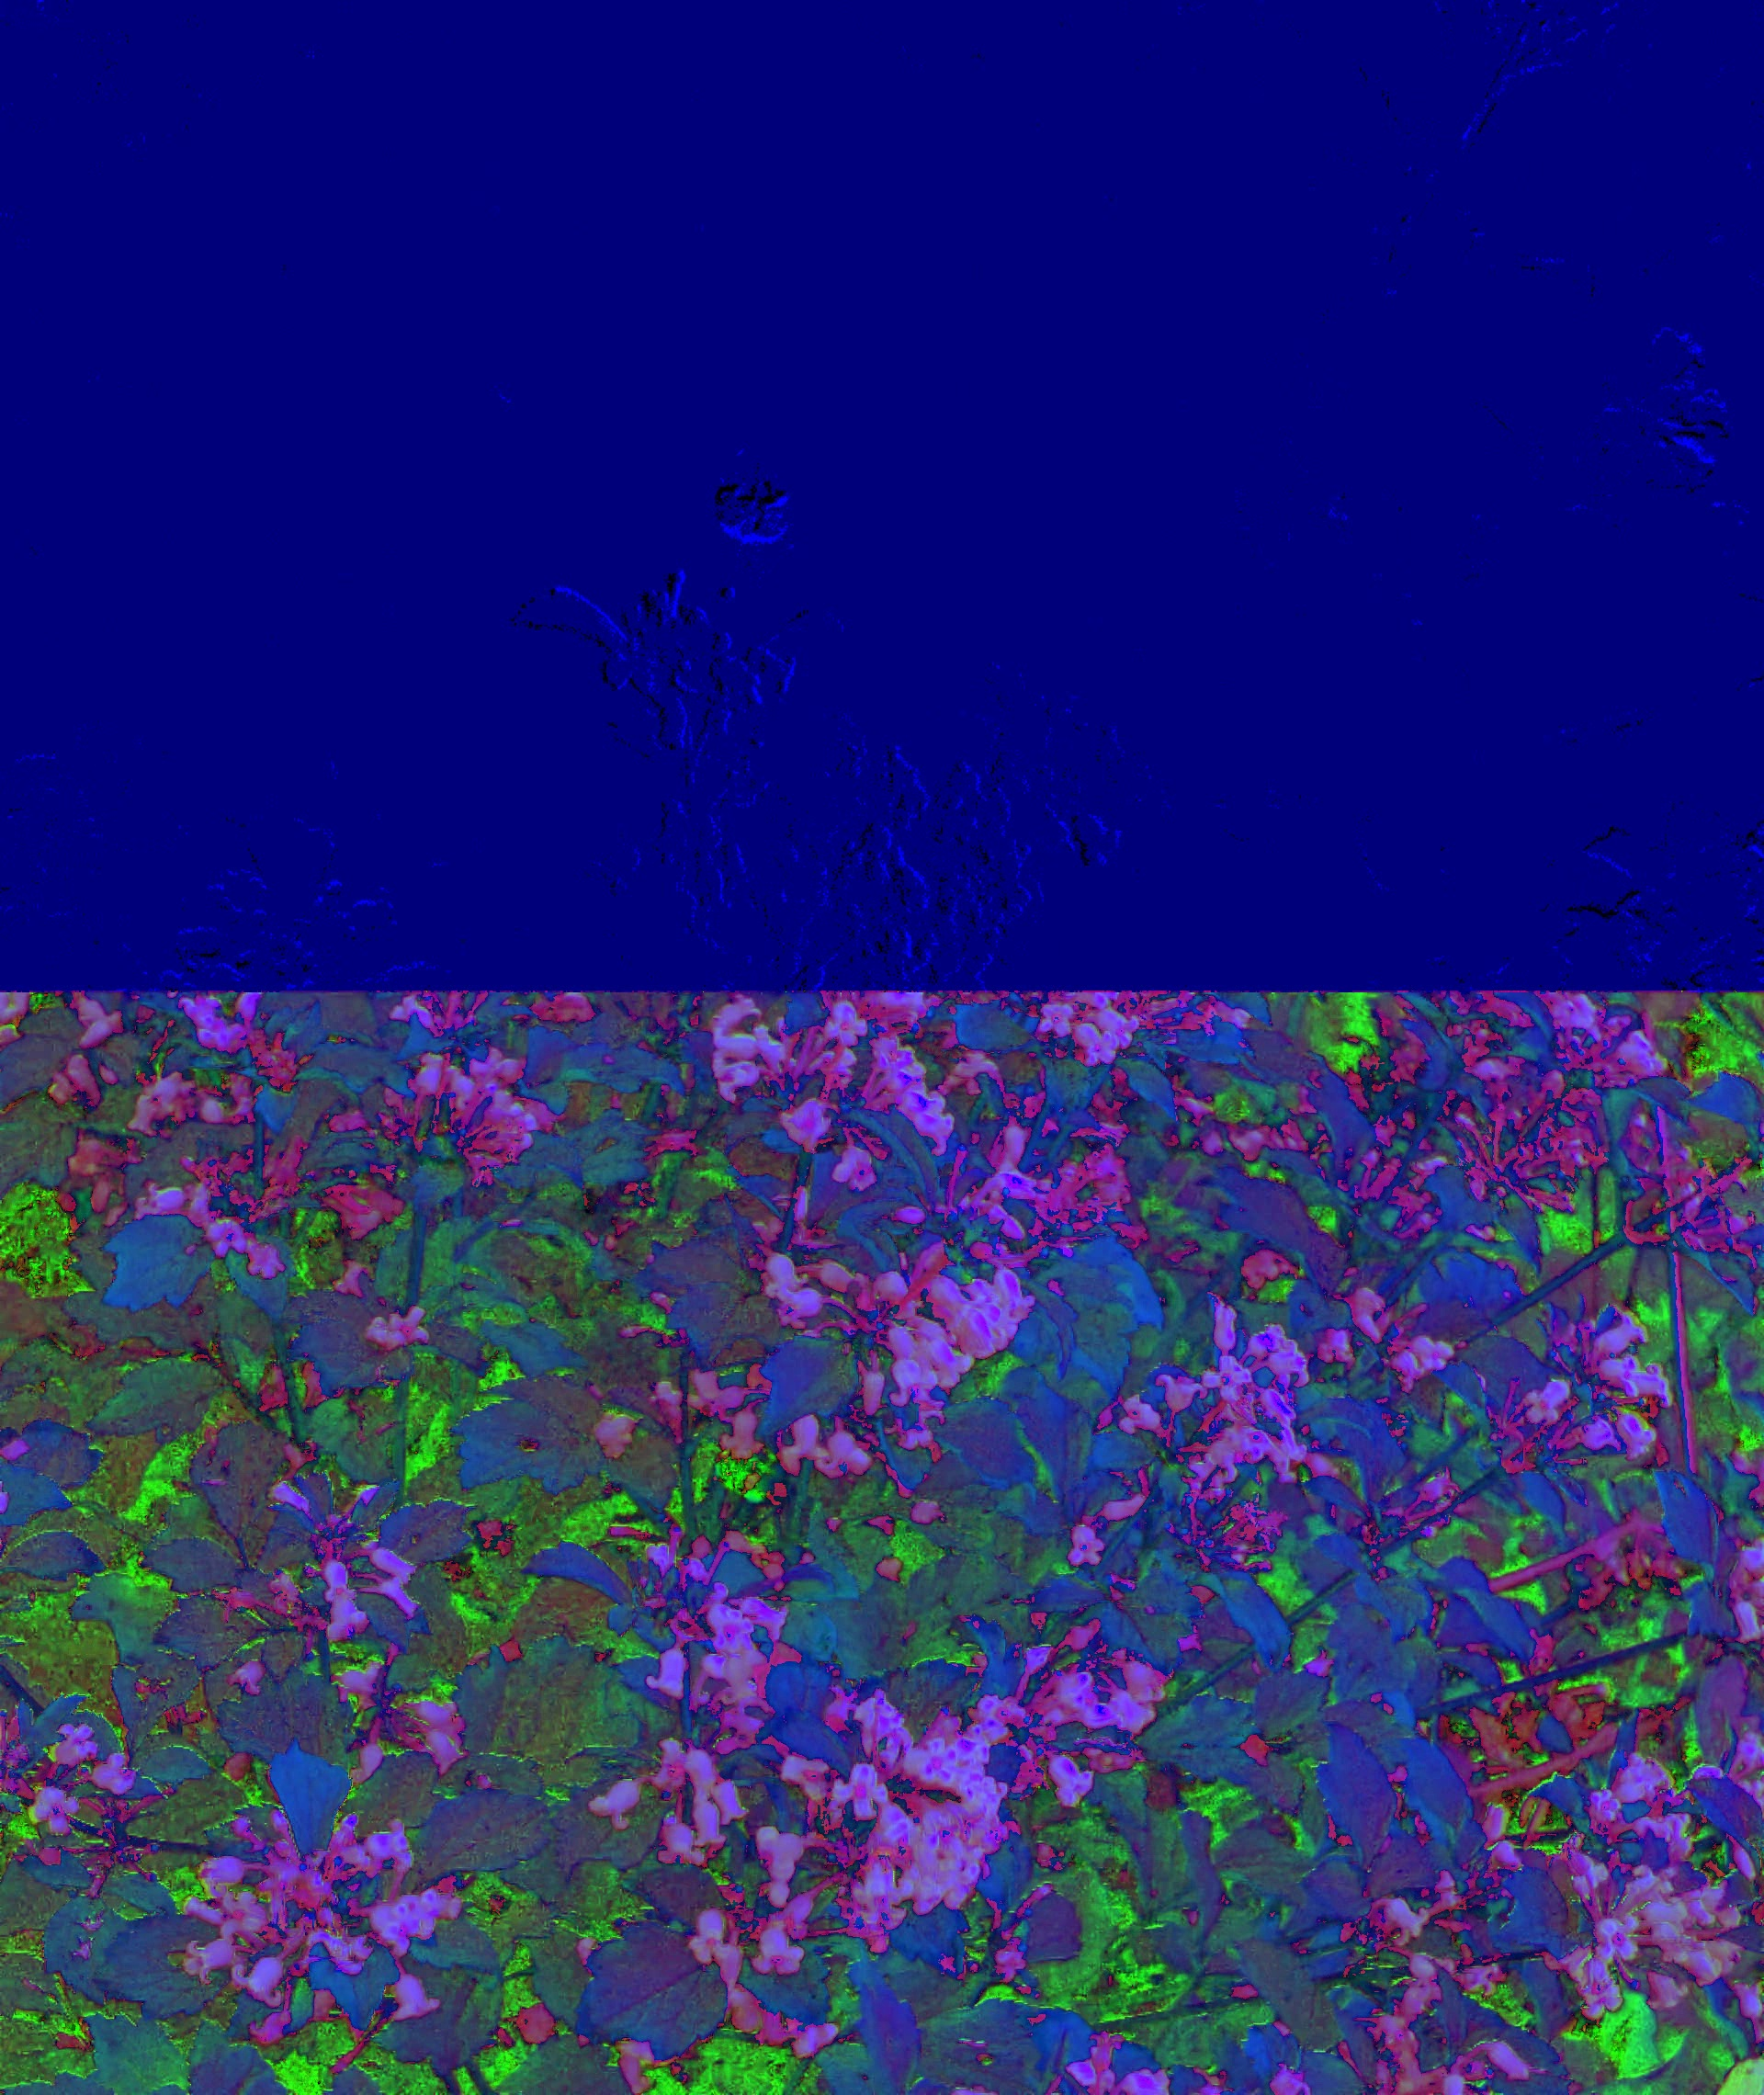
\includegraphics[width=\linewidth]{figures/preprocessings/hsv.jpg}
    \caption{RGB to HSV}
  \end{subfigure}
  \caption{Visual depiction of various preprocessing steps applied to the original stacked data set.}
  \label{fig:preprocessings}
\end{figure}
In the subsequent sections, each preprocessing method is introduced. The specific sequence of preprocessing steps employed for a given experiment will be elaborated upon in the results section.

\paragraph{Temporal Filtering}
\label{ch:pp-tf}
In our research, we employed a temporal filtering technique to process single-channel frame streams. This technique is governed by the following formula:

\[
out_i = {\left(1 - \frac{1}{fs}\right)} \times out_{i-1} + \frac{1}{fs \times in_i} 
\] 
Here, $fs$ denotes the filter size, indicating the weighting of previous frames considered in the filtering process. Throughout our experiments, we set $fs = 5$. The input to the filtering process, denoted as $in_i$, represents the selected input channel $k$ of the $i$th frame of the input video, structured as $M_{h\times w}$, where $h$ and $w$ correspond to the frame's height and width, respectively. The resulting output, $out_i$, also maintains the same dimensions, $M_{h\times w}$. \\
For initialization, we adopted the following configuration:

\[
out_0 = \begin{bmatrix}
0 & 0 & \cdots & 0 \\
0 & 0 & \cdots & 0 \\
\vdots & \vdots & \ddots & \vdots \\
0 & 0 & \cdots & 0 \\
\end{bmatrix}_{h \times w}
\]
This approach involves incorporating both, the current and the previous frames and accumulating them. Temporal dependent preprocessings are a common approach to increase the accuracy of insect detection models \cite{thiele2021towards}. The approach we employ diverges from a linear methodology; instead, it assigns significantly higher weights to the current and more recent frames compared to those further in the past. Specifically, the weighting scheme entails assigning a weight of $\frac{1}{fs}$ to the current frame, while the $p$-th previous frame (indexed as $i-p$) contributes to the output frame with a weight calculated as ${\left(1-\frac{1}{fs}\right)}^p \times \frac{1}{fs}$. This weighting mechanism ensures that the influence of past frames diminishes exponentially as they recede into the past. Consequently, frames closer to the present exert a stronger influence on the output frame, aligning with the temporal dynamics of the video stream (see Figure \ref{fig:tf}). We opted for $fs = 5$ to have a balance between maintaining a significant influence from frames with higher $p$ values and assigning considerably higher importance to frames nearer in time (see Figure \ref{fig:tf}). Such an approach aims to enrich the current frame with information from the recent past, enabling the capture of motion even when the subject remains static. This capability proves particularly valuable, for instance, in scenarios where insects exhibit minimal movement, ensuring that past motion remains accounted for.

\begin{figure}[H]
\begin{tikzpicture}
\begin{axis}[
axis lines = left,
    xlabel = \(p\),
    ylabel = {\(w(p)\)},
]
\addplot[color=black,domain=0:50]{(2/3)^x*1/3};
\addlegendentry{\(fs = 3\)}
\addplot[color=red,domain=0:50]{(4/5)^x*1/5};
\addlegendentry{\(fs = 5\)}
\addplot[color=blue,domain=0:50]{(9/10)^x*1/10};
\addlegendentry{\(fs = 10\)}
\addplot[color=green,domain=0:50]{(19/20)^x*1/20};
\addlegendentry{\(fs = 20\)}
\end{axis}
\end{tikzpicture}
\caption{Weights used in temporal filtering for different $fs$: $w(p) = {\left(1-\frac{1}{fs}\right)}^p \times \frac{1}{fs}$. Describing the decreasing impact of the previous frame to the output frame in temporal filtering approach.}
\label{fig:tf}
\end{figure}

\subsection{Setup cross validation}
To facilitate the cross-validation process, we established an infrastructure for each scene(totaling $n = 10$). An essential component of this infrastructure is a Bash script that iterates over the scenes, submitting the setup process to the Slurm\footnote{\url{https://slurm.schedmd.com/documentation.html}} task management tool on the computational unit. To improve performance, we implemented dependencies to ensure that only one split preparation process runs at any given time. This script also prepares the dependencies and parameters for the subsequent training process (see Section \ref{sec:training}). The setup of one cross-validation split encompasses several key tasks. Subsequently, bounding boxes are transformed from Labelbox format to the YOLO format \citep{wang2023yolov7}. Videos are then transformed into images of individual frames. For DVS, the upper part of the image is cropped. For DVS + RGB, each image gets undistorted using the respective camera calibration matrix \citep{zhang2000flexible}. The image is warped to map pixels of RGB frames to DSV frames \citep{glasbey1998review}. Then, from DVS and RGB four channels will be selected (this is configurable for the user) and merged into an RGBA frame. Frame extraction is implemented in Python using OpenCV \citep{bradski2000opencv}. Lastly, the script extracts the number of available cores on the hardware and leverages the Python multiprocessing framework to maximize hardware utilization. This involves processing a set of videos simultaneously to enhance efficiency. By executing these tasks, we establish a robust infrastructure for each scene, ensuring the seamless execution of cross-validation splits with optimized resource utilization.

\subsection{Train detection models using YOLO}
\label{sec:training}
In our experiments, we adhered to specific parameters and setup configurations. For a general workflow, we conducted training for 100 epochs. We implemented a patience of 25 epochs during training, whereby if there was no improvement in performance within this window, the training process was halted. Original image resolution was maintained to ensure comparability across experiment types. For the DVS experiment, we employed YOLOv8\footnote{\url{https://docs.ultralytics.com/de}}, utilizing the yolov8n model as the base for our training. An automatic batch size option determined a feasible batch size for the available hardware, while default hyperparameter configurations of YOLOv8 were applied. In the DVS + RGB experiment, YOLOv7 \citep{wang2023yolov7} was utilized with a modification to incorporate the Alpha Channel as input \citep{scharf2023TEMP}. A batch size of 96 was manually determined as optimal for hardware utilization. Training commenced with a pretrained model from \citeauthor{scharf2023TEMP}, chosen for its 4-channel architecture rather than the specific initialization weights. The default yolov7 configuration was applied for training parameters.

\subsection{Compare the results}

The validation of the data will be performed on the following criteria, each of which is measurable for each training of the data: We evaluate map@0.5 and map@0.5-0.95, as it is common in YOLO implementations. To assess the model's performance, we consider the best fitness over all epochs. For each validation split, we gather these metrics to obtain a distribution of Precision, Recall, map@0.5, and map@0.5-0.95 scores. To compare two preprocessings, we apply a paired $t$-Test to test if the mean of the differences $\mu_d$ is significantly different from 0. We apply an alternative hypothesis $H_A$ that assumes $\mu_d > 0$ to test directly for the better performance of a specific model. As input, we use the best fitness score of each validation split, a known method for comparing cross-validation results \citep{dietrich1998approximate}. The use of the $t$-Test comes with violations of the assumptions for $t$-Tests, as metric differences are not independent due to being calculated on the same dataset \citep{raschka2018model}. Despite drawbacks, especially the higher probability of false positives \citep{dietrich1998approximate}, other approaches are not feasible: \\ One-fold McNemar test \citep{dietrich1998approximate, raschka2018model} was not applicable, because different settings in each scene necessitate a test that validates performance across all scenes. The $5\times2$ validation method by \cite{dietrich1998approximate} was not feasible due to the 50\%/50\% split between test and validation data, which made the training set too small.


\section{Experiments}
\label{ch:experiments}
In our experiment naming scheme, we separate individual channels using underscores (\_). For each node in the preprocessing chain, we list the input and various preprocessing steps applied, separated by hyphens (--). If a preprocessing is applied to all channels, we group them within brackets. This scheme provides a concise and systematic way to represent the transformations applied to different channels in our research. The detailed abbreviations used to describe the components are listed in Table \ref{tbl:abbrs}. We will give a brief explanation of each experiment in this chapter.

\begin{table}[htb]
    \centering
    \begin{tabular}{c|l|l} 
        \textbf{Abbreviation} & \textbf{Type}          & \textbf{Explanation}        \\ 
        \hline
        DVS & \multirow{2}{*}{input} & DVS(Event)--Stream  \\
        RGB                      &                        & RGB(color)--Stream  \\ 
        \hline
        BS  & \multirow{3}{*}{preprocessing} & background subtraction  \\
        TF                      &                                  & temporal filtering \\
        HSV                      &                                  & RGB to HSV \\
        \hline
        R & \multirow{3}{*}{extraction} & extract red color \\
        G                    &                                & extract green color \\
        B                    &                                & extract blue color  \\
    \end{tabular}
    \caption{Different abbreviations and their explanations used in the experiments}
    \label{tbl:abbrs}
\end{table}
\subsection{Three channels}
Firstly we focused on using the DVS stream for insect detection. Therfore we used three channel RGB images as data base.
\label{ch:experiment-three}
\subsubsection{DVS\_DVS\_DVS (01)}
Here we tested the original videos, by using the DVS stream in all three image channels.
\subsubsection{DVS\_DVS--TF\_DVS (02)}
Here, we utilized the temporal filtering preprocessing for testing the impact of temporal filtering on original data. 

\subsubsection{DVS\_DVS--BS\_DVS-TF (03)}
We combined temporal filtering and background subtraction by applying both preprocessing on different channels while still maintaining the original DVS stream.
\subsubsection{DVS\_DVS--BS\_DVS--BS--TF (04)}
A variant of the previous attempt, where we applied the background subtraction to a temporal filtered DVS stream, rather than the original one. Figures \ref{fig:frame-comparison-original} and \ref{fig:frame-comparison-manipulated} demonstrate that this approach of preprocessing makes it easier to identify insects. Especially in the RGB stream at the bottom.

\begin{figure}[htbp] % You can specify the position of the figure (h: here, t: top, b: bottom, p: page)
    \centering % Center the image
    \includegraphics[width=\linewidth]{figures/preprocessings/extracted_frames/frame_03472_original.png} % Change 'example-image' to the filename of your image
    \caption{DVS and RGB frames stacked.} % Caption for the image
    \label{fig:frame-comparison-original} % A label to refer to the figure in the text
\end{figure}

\begin{figure}[htbp] % You can specify the position of the figure (h: here, t: top, b: bottom, p: page)
    \centering % Center the image
    \includegraphics[width=\linewidth]{figures/preprocessings/extracted_frames/frame_03472.png} % Change 'example-image' to the filename of your image
    \caption{Manipulated DVS and RGB frames stacked.} % Caption for the image
    \label{fig:frame-comparison-manipulated} % A label to refer to the figure in the text
\end{figure}

\subsection{HSV}
For all previous mentioned experiments (see Section \ref{ch:experiment-three}) we performed also an HSV transformation leading to the following four experiments:
\begin{itemize}
    \item (DVS\_DVS\_DVS)--HSV (05)
    \item (DVS\_DVS--TF\_DVS)--HSV (06)
    \item (DVS\_DVS--BS\_DVS--TF)--HSV (07)
    \item (DVS\_DVS--BS\_DVS--BS--TF)--HSV (08)
\end{itemize}
\subsection{Four channels}
For combining RGB and DVS stream we used a four channel approach with an additional alpha channel.
\subsubsection{RGB-R\_RGB-G\_RGB-G\_DVS (09)}
Here, we used all four possible input streams as the input to test the performance of the original data.
\subsubsection{DVS\_DVS--BS\_DVS--BS--TF\_RGB--BS (10)}
We per\-formed an experiment by combining the best DVS stream preprocessing approach with the best approach tested on the RGB data\footnote{This was performed and validated by another project group.}
\begin{table}[h]
\begin{tabular}{llc|r}
                                &                      & \textbf{ID} & \textbf{Name}   \\ \hline
\multirow{8}{*}{\rotatebox[origin=c]{90}{3-Channels}} & \multirow{4}{*}{\rotatebox[origin=c]{90}{RGB}} & 01                           & DVS\_DVS\_DVS                    \\
                                &                      & 02                           & DVS\_DVS--TF\_DVS                \\
                                &                      & 03                           & DVS\_DVS--BS\_DVS-TF             \\
                                &                      & 04                           & DVS\_DVS--BS\_DVS--BS--TF        \\ \cline{2-4} 
                                & \multirow{4}{*}{\rotatebox[origin=c]{90}{HSV}} & 05                           & (DVS\_DVS\_DVS)--HSV             \\
                                &                      & 06                           & (DVS\_DVS--TF\_DVS)--HSV         \\
                                &                      & 07                           & (DVS\_DVS--BS\_DVS--TF)--HSV     \\
                                &                      & 08                           & (DVS\_DVS--BS\_DVS--BS--TF)--HSV \\ \hline
\multirow{2}{*}{\rotatebox[origin=c]{90}{4-}}  & \multirow{2}{*}{}    & 09                           & RGB-R\_RGB-G\_RGB-B\_DVS         \\
                                &                      & 10                           & DVS\_DVS--BS\_DVS--BS--TF\_RGB--BS
\end{tabular}
\caption{Assignment of experiment name to IDs. Used in later sections for better readability.}
\label{tbl:assign-experiment-id}
\end{table}

\section{Results}
\begin{figure*}
    \centering
    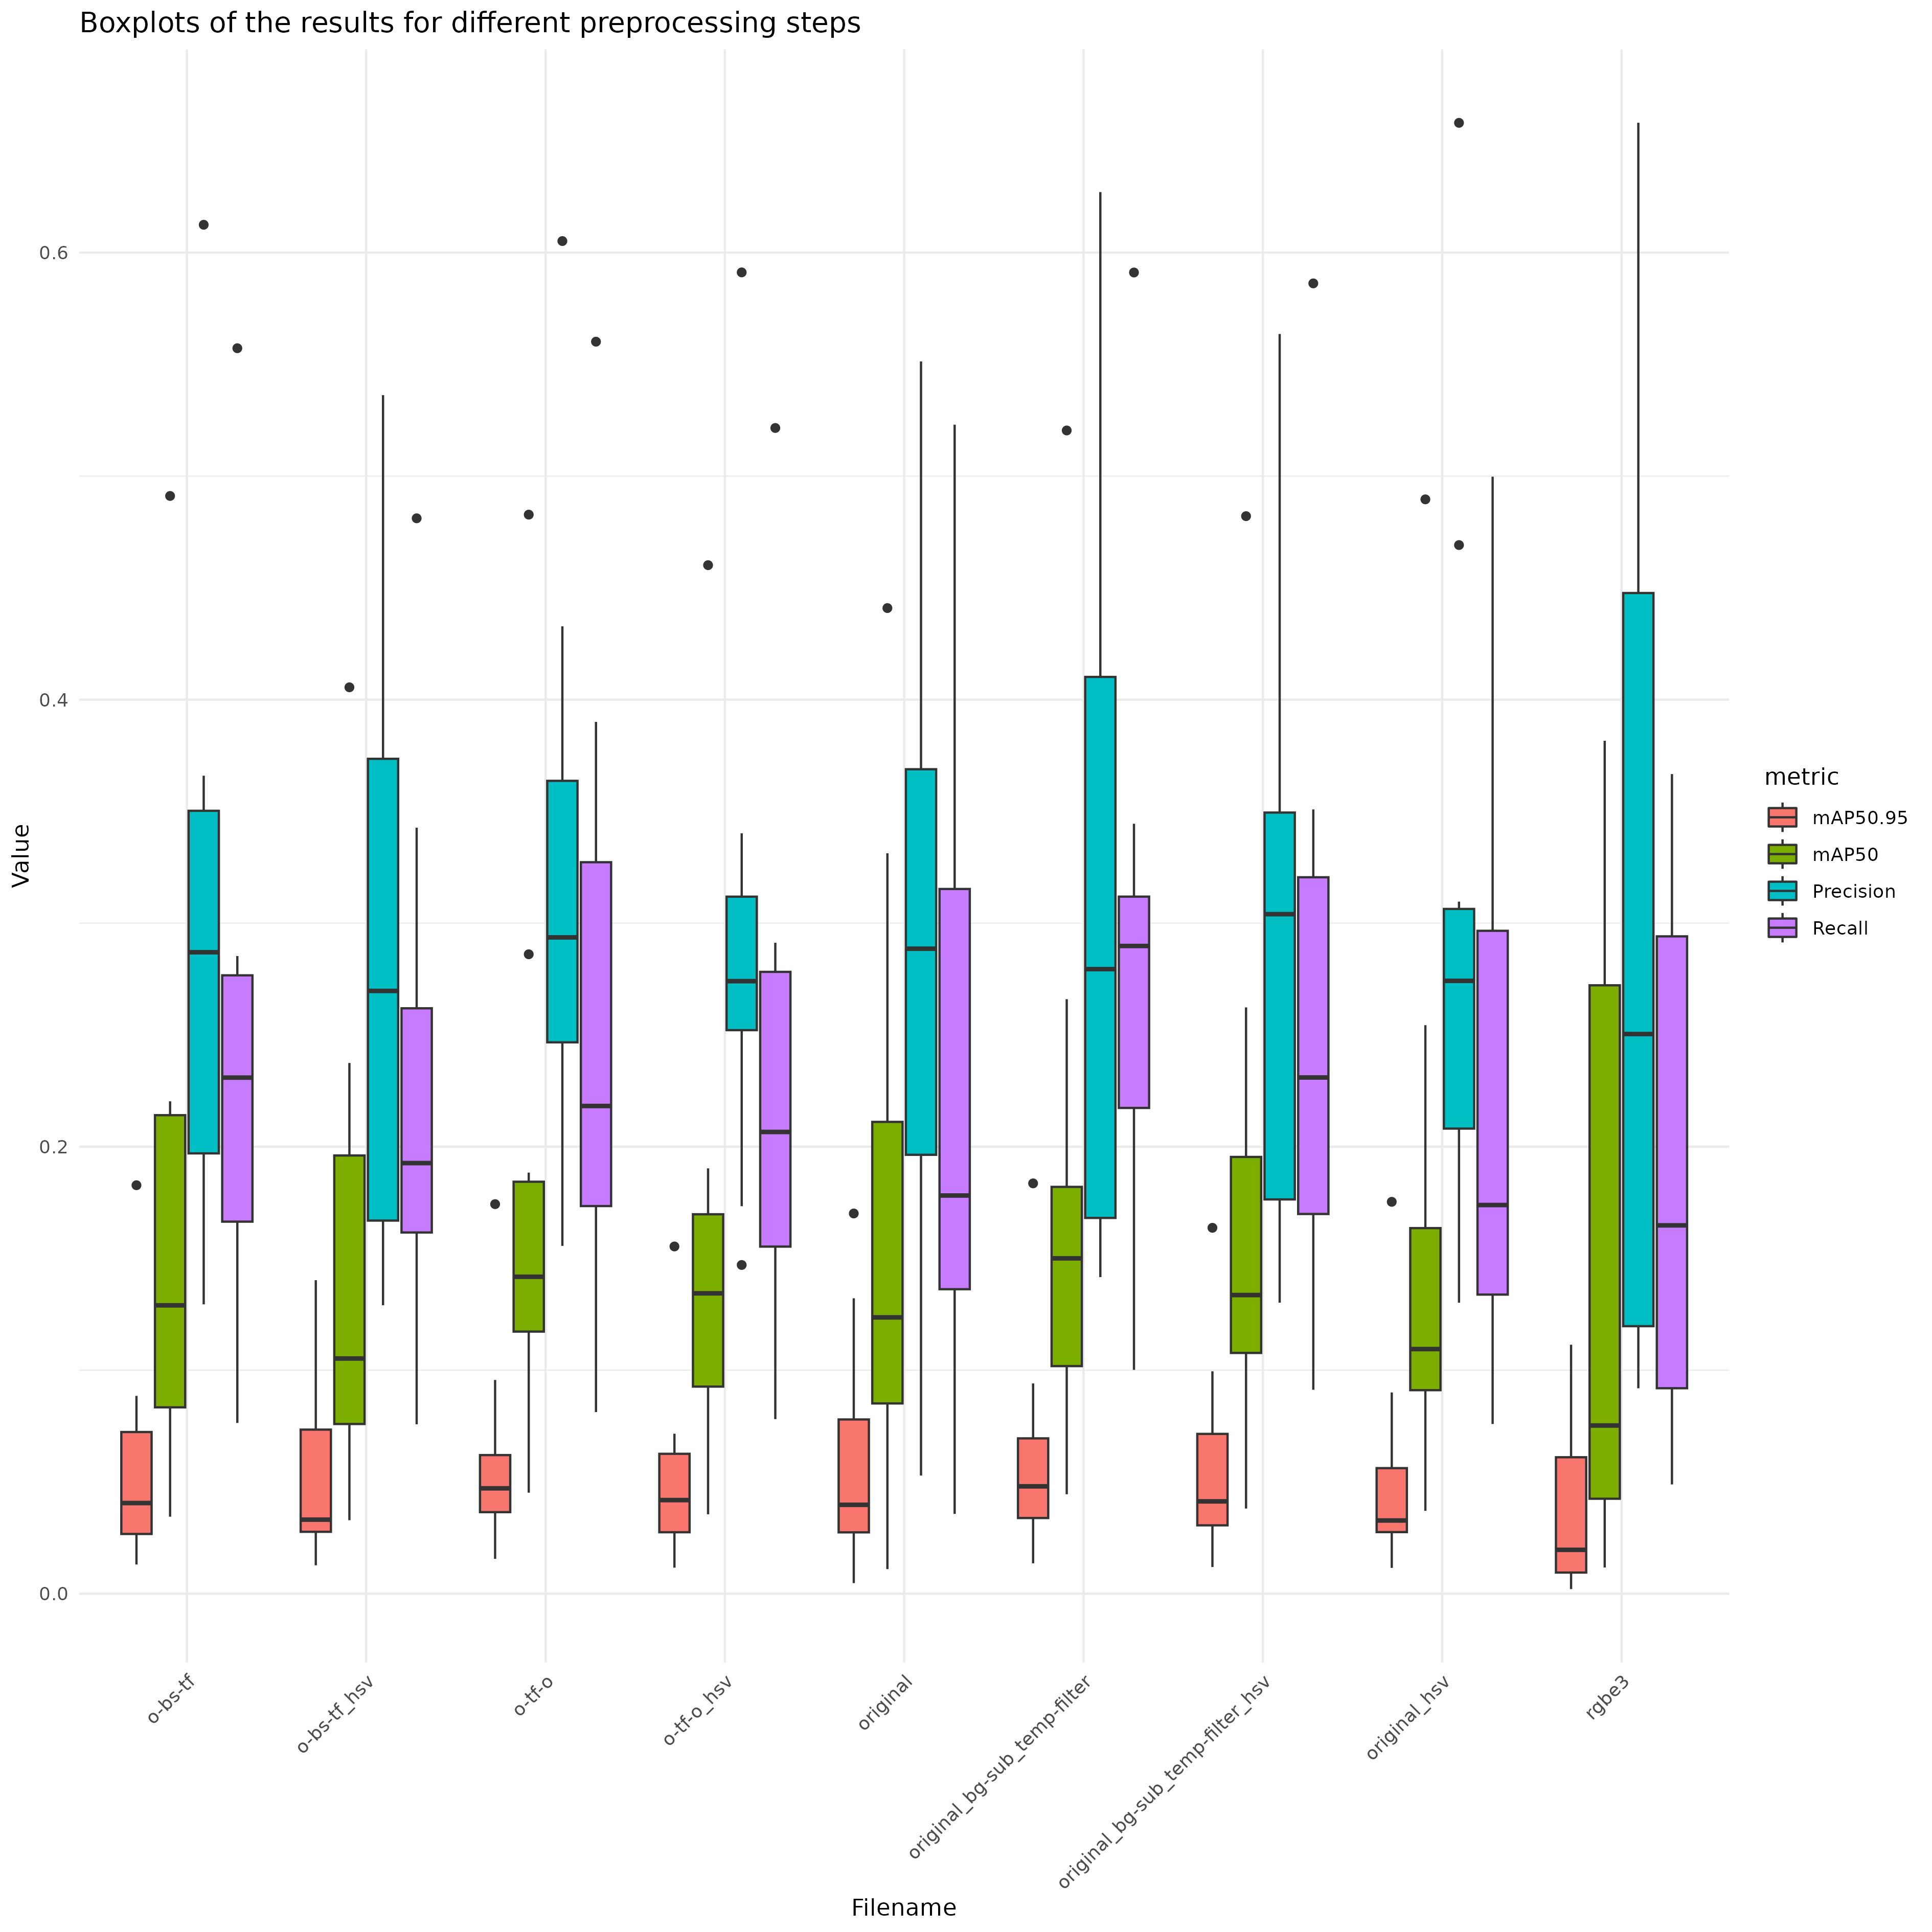
\includegraphics[width=\textwidth]{figures/results/boxplots/overview.png}
    \caption{Boxplots describing the distribution of different metrics measured in the described experiments. Experiments are ordered and labelled as introduced in Section \ref{ch:experiments}.}
    \label{fig:results:overview}
\end{figure*}


\subsection{Precision}
In Experiment 08, the mean precision attained was 0.279, with a median value of 0.269 (see Figure \ref{fig:results:overview}). Conversely, Experiment 04, incorporating HSV preprocessing, demonstrated a slightly higher mean precision of 0.294, with a similar median value of 0.287 (see Figure \ref{fig:results:overview}). These findings suggest that the inclusion of HSV preprocessing did not substantially affect precision compared to the configuration without it. Similarly, Experiment 06 yielded a mean precision of approximately 0.293, while Experiment 02 achieved a slightly higher mean precision of 0.317. Both configurations exhibited comparable median precision values, indicating consistent performance despite the addition of HSV preprocessing. Notably, Experiment 10, employing RGB preprocessing, showcased a significantly higher mean precision of about 0.360 compared to Experiments 08 and 04, which achieved mean precisions of 0.297 and 0.306, respectively. This indicates that RGB preprocessing may have a more pronounced positive impact on precision within this experimental context. Furthermore, when comparing Experiment 01 and Experiment 05, marginal differences in mean precision were observed, with values of 0.321 and 0.301, respectively, suggesting that the inclusion of HSV preprocessing did not substantially alter precision outcomes. Lastly, Experiment 09 exhibited the highest mean precision among all configurations, at 0.340, indicating the potential efficacy of RGB preprocessing in enhancing precision metrics compared to configurations solely within the DVS framework.

\subsection{Recall}
The findings from the experiments conducted demonstrate varying levels of recall across different configurations. Experiment 08, for instance, yielded a mean recall of 0.222, with values ranging from 0.076 to 0.481, and a median of 0.193. In comparison, Experiment 04 exhibited a slightly higher mean recall of 0.240, with values ranging from 0.076 to 0.557, and a median of 0.231. Similarly, Experiment 06 and Experiment 02 displayed mean recalls of 0.230 and 0.254 respectively, with corresponding maximum, minimum, and median values. Notably, Experiment 10, which employed RGB preprocessing, showed a significantly higher mean recall of approximately 0.281, compared to Experiments 08 and 04, which utilized HSV preprocessing, with mean recalls around 0.254 and 0.280 respectively. This discrepancy suggests a potentially more pronounced positive impact of RGB preprocessing on recall within this experimental framework. Furthermore, marginal differences in mean recall were observed between Experiment 01 and Experiment 05 configurations, with both hovering around 0.224. The disparities in maximum, minimum, and median values between these configurations were negligible. Lastly, Experiment 09 displayed the lowest mean recall among all configurations, approximately 0.196, indicating that RGB preprocessing may not have as significant a positive effect on recall when compared to configurations solely within the DVS framework.

% Define colors
\definecolor{color1}{RGB}{166,206,227}
\definecolor{color2}{RGB}{31,120,180}
\definecolor{color3}{RGB}{178,223,138}
\definecolor{color4}{RGB}{51,160,44}
\definecolor{color5}{RGB}{251,154,153}
\definecolor{color6}{RGB}{227,26,28}
\definecolor{color7}{RGB}{253,191,111}
\definecolor{color8}{RGB}{255,127,0}
\definecolor{color9}{RGB}{202,178,214}
\definecolor{color10}{RGB}{106,61,154}

\begin{filecontents}{data.dat}
x      y1         y2         y3         y4         y5         y6        y7         y8         y9         y10       x1
1      0.103068   0.071699   0.028952   0.005158   0.038149   0.03305   0.031572   0.033066   0.057206   0.03562   1
2      0.217274   0.111262   0.042605   0.013288   0.063355   0.039304   0.044736   0.020577   0.081338   0.018906   2
3      0.192223   0.043366   0.076576   0.016691   0.057421   0.031058   0.042065   0.029824   0.055887   0.028706   3
4      0.173852   0.064634   0.058356   0.013779   0.055287   0.028051   0.039459   0.021871   0.054134   0.024501   4
5      0.190506   0.063821   0.058298   0.015873   0.05333   0.030592   0.036943   0.022816   0.050228   0.034788   5
6      0.213286   0.064507   0.050526   0.01247   0.056628   0.025518   0.035376   0.025362   0.046521   0.035608   6
7      0.183555   0.055202   0.053262   0.012333   0.05693   0.027898   0.034199   0.025655   0.048242   0.035436   7
8      0.182981   0.061142   0.047545   0.01326   0.05667   0.025225   0.034053   0.026015   0.04565   0.034474   8
9      0.179159   0.055973   0.0527   0.012952   0.057655   0.024271   0.035664   0.027539   0.044777   0.034764   9
10      0.181054   0.054132   0.053788   0.012357   0.057444   0.023383   0.036436   0.026919   0.045214   0.036432   10
11      0.181788   0.055331   0.054346   0.011734   0.056909   0.022718   0.036622   0.027226   0.044277   0.036843   11
12      0.18568   0.056338   0.053821   0.011665   0.056478   0.023099   0.036765   0.026538   0.043631   0.036617   12
13      0.188243   0.056929   0.054391   0.011845   0.055516   0.023314   0.03745   0.024142   0.043432   0.037699   13
14      0.189183   0.056661   0.054517   0.012172   0.055625   0.023789   0.037878   0.023222   0.043665   0.037907   14
15      0.188849   0.05787   0.054415   0.012519   0.055162   0.023303   0.038409   0.022712   0.044932   0.037971   15
16      0.186295   0.059608   0.054643   0.012979   0.055441   0.023587   0.037971   0.022099   0.04549   0.038373   16
17      0.184302   0.060418   0.054986   0.013277   0.055398   0.023147   0.038036   0.022936   0.045879   0.038586   17
18      0.181363   0.060555   0.056115   0.013556   0.055263   0.02273   0.038216   0.02481   0.046912   0.038521   18
19      0.178705   0.059629   0.055336   0.014017   0.055196   0.0227   0.039259   0.024463   0.047193   0.039372   19
20      0.179251   0.058748   0.054959   0.014366   0.055531   0.022482   0.039399   0.025242   0.046493   0.039517   20
21      0.17723   0.058866   0.055915   0.014705   0.055949   0.022038   0.039644   0.025571   0.046763   0.039474   21
22      0.178178   0.058657   0.056578   0.01508   0.056298   0.021849   0.041823   0.025969   0.04735   0.039956   22
23      0.177433   0.058646   0.057003   0.015397   0.056936   0.021677   0.041782   0.026126   0.04768   0.040001   23
24      0.175565   0.058322   0.058161   0.015559   0.057261   0.021667   0.04184   0.026223   0.04768   0.040507   24
25      0.177295   0.057253   0.059366   0.015614   0.057345   0.021621   0.042104   0.026563   0.047538   0.040677   25
26      0.178305   0.056295   0.059828   0.015568   0.057245   0.021216   0.041553   0.026356   0.048113   0.040719   26

\end{filecontents}

\begin{figure*}
    \centering
    \begin{tikzpicture}
        \begin{axis}[
            axis lines = left,
            width = 0.95\textwidth,
            height = 0.5\textwidth,
            legend style={font=\small,at={(1,0.532)},anchor=east},
            xlabel={Epoch},
            ylabel={$0.1 \times \text{map@0.5} + 0.9 \times \text{map@0.5--0.95}$},
        ]
            \addplot[color1] table [x=x, y=y1] {data.dat};
            \addlegendentry{2023-09-28\_12-16-27}
            
            \addplot[color2] table [x=x, y=y2] {data.dat};
            \addlegendentry{2023-09-28\_12-24-48}
        
            \addplot[color3] table [x=x, y=y3] {data.dat};
            \addlegendentry{2023-09-30\_15-28-40}
        
            \addplot[color4] table [x=x, y=y4] {data.dat};
            \addlegendentry{2023-10-01\_13-59-10}
            \addplot[color5] table [x=x, y=y5] {data.dat};
            \addlegendentry{2023-10-01\_14-05-35}
            \addplot[color6] table [x=x, y=y6] {data.dat};
            \addlegendentry{2023-10-10\_12-47-19}
            \addplot[color7] table [x=x, y=y7] {data.dat};
            \addlegendentry{2023-10-10\_12-51-16}
            \addplot[color8] table [x=x, y=y8] {data.dat};
            \addlegendentry{2023-10-10\_12-51-16}
            \addplot[color9] table [x=x, y=y9] {data.dat};
            \addlegendentry{2023-10-10\_14-00-44}
            \addplot[color10] table [x=x, y=y10] {data.dat};
            \addlegendentry{2023-10-11\_15-18-06}
        
        \end{axis}
    \end{tikzpicture}
    \caption{Evolution of fitness values along the epochs, in cross-validation of experiment 04.}
    \label{fig:fitness-experiment04}
\end{figure*}


The outcomes of various experimental configurations highlight the variability in mean mAP@0.5 values. Experiment 08, for instance, demonstrated a mean mAP@0.5 of 0.147, with values ranging from 0.033 to 0.406, and a median of 0.105. Conversely, Experiment 04 exhibited a slightly higher mean mAP@0.5 of 0.167, with values ranging from 0.034 to 0.491, and a median of 0.129. Similarly, Experiment 06 and Experiment 02 yielded mean mAP@0.5 values of approximately 0.156 and 0.179 respectively, with corresponding maximum, minimum, and median values. A significant difference was noted between Experiment 10 and Experiment 08/04 configurations. The former, integrating RGB preprocessing, showcased a mean mAP@0.5 of approximately 0.205, compared to the latter, which displayed mean mAP@0.5 values around 0.171/0.180. This suggests a potentially more pronounced positive impact of RGB preprocessing on mAP@0.5 within this experimental context. Furthermore, when comparing Experiment 01 and Experiment 05 configurations, marginal differences in mean mAP@0.5 were observed, along with negligible discrepancies in maximum, minimum, and median values. Lastly, the Experiment 09 configuration exhibited the lowest mean mAP@0.5 among all configurations, approximately 0.150, indicating that RGB preprocessing may not have as significant a positive effect on mAP@0.5 when compared to configurations solely within the DVS framework.

\subsection{mAP@0.5--0.95}
Experiment 08 resulted in a mean mAP@0.5--0.95 of 0.053, with values ranging from 0.013 to 0.140 and a median of 0.033. Conversely, Experiment 04 displayed a slightly higher mean mAP@0.5--0.95 of 0.059, with values ranging from 0.013 to 0.183 and a median of 0.041. Similarly, Experiment 06 showed a mean mAP@0.5--0.95 of approximately 0.053, with values ranging from 0.012 to 0.155 and a median of 0.042, while Experiment 02 yielded a slightly higher mean mAP@0.5--0.95 of 0.060, with values ranging from 0.016 to 0.174 and a median of 0.047 (refer to Figure \ref{fig:results:overview}). A notable difference was observed between Experiment 10 and Experiment 08/04 configurations. The former, integrating RGB preprocessing, demonstrated a mean mAP@0.5--0.95 of approximately 0.059, with values ranging from 0.012 to 0.183 and a median of 0.037, compared to the latter, which exhibited mean mAP@0.5--0.95 values of around 0.058/0.059. Their respective values ranged from 0.164/0.184 to 0.012/0.014, with medians of 0.041/0.048 (refer to Figure \ref{fig:results:overview}). This suggests that RGB preprocessing may exert a more pronounced positive impact on mAP@0.5--0.95 compared to HSV preprocessing within this experimental context. Furthermore, when comparing Experiment 01 and Experiment 05 configurations, marginal differences in mean mAP@0.5--0.95 were observed, with values of approximately 0.052 and 0.056 respectively. The maximum, minimum, and median values also exhibited negligible discrepancies between these configurations. Lastly, Experiment 09 exhibited the lowest mean mAP@0.5--0.95 among all configurations, approximately 0.036, with values ranging from 0.002 to 0.120 and a median of 0.019. This suggests that RGB preprocessing may have a less pronounced positive effect on mAP@0.5--0.95 compared to configurations solely within the DVS framework.

\subsection{Comparison}
\begin{table}[h]
\begin{tabular}{c|*{9}{c}}
 &  10 & 02 & 03 & 08 & 01 & 06 & 07 & 05 & 09 \\
\hline
04 &  \textcolor{red}{.491} & \textcolor{red}{.342} & \textcolor{red}{.117} & \textcolor{red}{.116} & \textcolor{green}{.048} & \textcolor{green}{.029} & \textcolor{green}{.041} & \textcolor{green}{.010} & \textcolor{green}{.008} \\
10 &  NA & \textcolor{red}{.447} & \textcolor{red}{.333} & \textcolor{red}{.358} & \textcolor{red}{.226} & \textcolor{red}{.136} & \textcolor{red}{.154} & \textcolor{red}{.176} & \textcolor{green}{.030} \\
02 &  NA & NA & \textcolor{red}{.296} & \textcolor{red}{.220} & \textcolor{green}{.027} & \textcolor{green}{.019} & \textcolor{red}{.051} & \textcolor{green}{.001} & \textcolor{green}{.001} \\
03 &  NA & NA & NA & \textcolor{red}{.472} & \textcolor{red}{.166} & \textcolor{red}{.057} & \textcolor{red}{.094} & \textcolor{red}{.063} & \textcolor{green}{.013} \\
08 &  NA & NA & NA & NA & \textcolor{red}{.116} & \textcolor{red}{.077} & \textcolor{green}{.043} & \textcolor{green}{.023} & \textcolor{green}{.003} \\
01 &  NA & NA & NA & NA & NA & \textcolor{red}{.158} & \textcolor{red}{.195} & \textcolor{red}{.109} & \textcolor{green}{.003} \\
06 &  NA & NA & NA & NA & NA & NA & \textcolor{red}{.462} & \textcolor{red}{.421} & \textcolor{green}{.014} \\
07 &  NA & NA & NA & NA & NA & NA & NA & \textcolor{red}{.462} & \textcolor{green}{.016} \\
05 &  NA & NA & NA & NA & NA & NA & NA & NA & \textcolor{green}{.021} \\
\end{tabular}

\caption{Analyzing $t$-Test Results, by comparing the distribution of maximum fitness values across cross-validation elements. The rows and columns are arranged in descending order based on the mean of each experiment. The null hypothesis ($H_0$) posits that the true mean difference between the column value and the row value is not greater than zero, while the alternative hypothesis ($H_A$) suggests that the true mean difference is greater than zero. Cells are color-coded green if $H_0$ can be rejected at a significance level of $\alpha = .05$, indicating statistical significance; otherwise, they are colored red.}
\label{tbl:result-comparison}
\end{table}

Experiment 04 emerges as the top performer overall, boasting the highest mean fitness value among all experiments. Notably, it surpasses the original DVS stream (Experiment 01) with statistical significance. However, the introduction of RGB background subtraction in Experiment 04 does not yield a significant impact, as evidenced by the comparison with Experiment 10 in Table \ref{tbl:result-comparison}. Conversely, the amalgamation of the original RGB and DVS streams in Experiment 09 demonstrates inferior performance compared to all other experiments, as indicated in Table \ref{tbl:result-comparison}. Furthermore, the incorporation of temporal filtering to the DVS stream, as observed in experiment 02, leads to a significant enhancement in results relative to experiment 01. While overall HSV appears to underperform compared to corresponding RGB experiments, RGB does not exhibit significantly higher means, except in the case of experiments 02 and 06.

\section{Discussion}
- Using RGB backgrouund subtraction as additional information, has no impact.
    - Further analysis on RGB impacts needs to implemented. \\

In this study, we explored the feasibility of detecting tiny insects in cluttered environments using RGB and DVS-event stream images. The results we found not only show that this kind of detection is possible, but they also show how complex environments affect the complex link between preprocessing methods and detection success.\\
The use of temporal-based preprocessing approaches appeared as an important component in our research. By leveraging temporal filtering, we were able to isolate non-moving insects within DVS streams, thereby reducing the impact of background noise and enhancing the clarity of insect-related motion patterns. This finding underscores the importance of considering temporal dynamics in the preprocessing pipeline for insect detection tasks.\\
Our experiments utilizing background subtraction techniques produced promising results. By applying background subtraction, we successfully delineated moving insects from stationary background elements, such as plants. This preprocessing step not only facilitated the extraction of relevant motion features but also contributed to the mitigation of false positives, thus improving overall detection accuracy.\\
However, despite the efficacy of temporal-based and background subtraction preprocessings, our analysis revealed the susceptibility of detection outcomes to various environmental factors. Factors such as the size of insects, the presence of non-insect objects in the scene, and the speed of movement of these objects exerted significant influences on detection performance. Addressing these challenges necessitates the development of robust preprocessing strategies capable of adapting to diverse environmental conditions.\\
While temporal-based techniques exhibited substantial improvements in detection accuracy, the impact of the HSV transformation on model outcomes was relatively minimal. This observation suggests that color space transformations may have limited utility in certain insect detection scenarios, highlighting the need for careful consideration of preprocessing techniques based on the specific characteristics of the input data.\\
Our investigation into the effects of incorporating RGB background subtraction as supplementary information yielded intriguing insights. Even though this preprocessing step didn't seem to improve the results of our tests, more research is needed to fully understand how it might have affected the results. Future research efforts should explore alternative approaches to leveraging RGB information effectively in insect detection tasks, considering its potential significance in other contexts.\\
In conclusion, our study contributes to the growing body of research on insect detection by showcasing the effectiveness of preprocessing techniques in enhancing detection accuracy in challenging environments.

\section{Limitations}

Despite the promising potential of our approach, several limitations must be acknowledged. The relatively small size of the dataset used for training and validation poses a primary constraint, potentially limiting the generalization capability of machine learning models and increasing the risk of overfitting, particularly in diverse natural environments where insect populations and behaviors may vary significantly. Moreover, while efforts were made to ensure accurate manual labeling of the dataset, the inherent complexity of insect behavior and the intricacies of outdoor environments may introduce uncertainties and biases into the annotations. Variations in annotator interpretation, labeling consistency, and the inherent subjectivity involved in identifying and categorizing insect species could impact the performance of trained models, potentially leading to suboptimal detection and tracking results. 
Moreover, the suitability of single-stage CNNs like YOLO for detecting small objects, such as insects, is a concern, as these architectures may struggle with accurately capturing the small size and rapid motion of insects in cluttered outdoor environments
Thus, while our study provides valuable insights into the potential of machine learning for insect monitoring, further research and refinement in dataset collection, and model development are necessary to address these challenges effectively and enhance the robustness and applicability of insect monitoring technologies in real-world scenarios.

\section{Further Works}
Utilizing the same YOLO version and configuration throughout experiments is imperative for ensuring consistency and comparability. We employed both YOLO versions 7 and 8 to facilitate this objective. While most experiments were conducted within a three-channel environment, further exploration into the impact of additional RGB input on the fourth channel is warranted. Detailed testing in this regard could provide deeper insights into the implications of utilizing the alpha channel as a YOLO input channel. Experiment 10, which combines DVS results with RGB results, allocated only one channel for the RGB stream. However, three-channel approaches exist within the RGB domain. One potential solution could involve employing leave-one-out cross-validation, thereby disregarding two of the six input bands from DVS and RGB for the experiment. Default hyperparameters were utilized in our experiments. Maximizing the hyperparameter space could potentially enhance results further. The choice of a qualitative metric for selecting a $fs$ value for temporal filtering was employed in our experiments. Adopting a more quantitative setup, such as comparing detection metrics for different $fs$ values in preprocessing, could validate the quality of this choice. The field of computer vision offers numerous other preprocessing possibilities beyond those explored in our experiments. Non-AI-based object detection processes, in particular, could be investigated for their efficacy in preprocessing. Low batch sizes have not been extensively studied in object detection problems \cite{Peng_2018_CVPR}. Exploring the influence of different batch sizes on results could shed light on their impact and potential for improving generalization.
\section{Conclusion}

\begin{acks}
  Calculations (or parts of them) for this publication were performed on the HPC cluster PALMA II of the University of Münster, subsidised by the DFG (INST 211/667-1).
\end{acks}

\bibliographystyle{ACM-Reference-Format}
\bibliography{sample-base}
\pagebreak
%%
%% If your work has an appendix, this is the place to put it.
%\appendix
\appendix

\section{Individual reports}
- Research
    - Evaluation metrics
    - Yolo version differences
    - Preprocessings
    - Cross-validations
    - Compare cross-validations
- Implementation
    - Labelbox to Yolo Format
        - Video to frame
        - JSON to txt labels
        - Splitting dataset between val and train
    - Preprocessing
        - Framework for utilizing preprocessings on all videos
            - Preprocess all channels of a image ombined
            - Fine grained processing of only selected input channels, pushed to explicit output channells
        - Implement different preprocessings.
            - (Hier Liste mit allen PP einfügen [auch wenn nicht genutzt mMn])
        - Multithreading of preprocessing videos and building datasets
        - Calls to APIs of different YOLO versions to use their train functions
        - Init a cross validation, by defining scripts for each cross-validation step, which than can be executed on HPC-Cluster.
        - Submit the scripts on correct partitions automatically and introducing logical dependencies.
        - Debugging yolov7
        - Undistort and transform pixels, for mapping RGB stream to DVS stream.
        - Infrastructure for defining inputs in RGBA experiments.
        - Evalutae the results
            - Summarize best epochs for each cross-validation in csv files
            - Visualize results
            - normalize result reporting of v7 and v8 of yolo.
            - Utilize testing utilities for compare cross-validations
- Project Managment
    - Define data structruing
    - Listing project steps
    - Documentation
- Monitoring PALMA processes
    - Monitor if the runs work as expected
    - Fine tune hardware usages, for better overall utilzation of HPC hardware.
\subsection{Fred}
\subsection{Jakob}

% Define a macro to escape underscores
\newcommand{\escapeunderscore}[1]{%
    \StrSubstitute{#1}{_}{\string_}%
}
\newcommand{\substringtwenty}[1]{\StrMid{#1}{2}{11}}

\newcommand{\escapeunderscoreandsubstring}[1]{%
    \StrSubstitute{#1}{_}{\string_}[\temp]% Escape underscores
    \StrMid{\temp}{2}{20}% Extract substring
}

\newcommand{\customcsvtableEight}[2]{
    \subsection{#2}
    \begin{table}[H]
        \centering
        
        \begin{longtable*}{c|c|c|c|c|c|c|c|cc}
        \multirow{2}{*}{} &
        \multicolumn{1}{c}{}  & \multicolumn{4}{|c|}{Metrics} & \multicolumn{3}{|c}{Validation Loss} \\
        Name & Epoch & Precision & Recall & mAP@0.5 & mAP@0.5-0.95 & Box & Cls & Dfl & \\
        \hline
        \csvreader[
            separator=comma
        ]{#1}{}{
       \escapeunderscoreandsubstring{\csvcolxvi} & \csvcolii & \csvcolvi & \csvcolvii & \csvcolviii & \csvcolix & \csvcolx & \csvcolxi & \csvcolxii \\
        }
    \end{longtable*}
     \caption{Cross-validation results of experiment #2. For each validation split the epoch with best fitness and the respective metrics and validation loss is listed.}
       
    \end{table}
}
\newcommand{\removequotes}[1]{%
    \StrSubstitute{#1}{"}{}%
}
\newcommand{\customcsvtablevSeven}[2]{
    \subsection{#2}
    \begin{table}[H]
        \centering
        
        \begin{longtable*}{c|c|c|c|c|c|c|c|cc}
        \multirow{2}{*}{} &
        \multicolumn{1}{c}{}  & \multicolumn{4}{|c|}{Metrics} & \multicolumn{3}{|c}{Validation Loss} \\
        Name & Epoch & Precision & Recall & mAP@0.5 & mAP@0.5-0.95 & Box & Cls & Dfl & \\
        \hline
        \csvreader[
            separator=comma
        ]{#1}{}{
       \escapeunderscoreandsubstring{\csvcolxxiii} & \csvcoliii & \removequotes{\csvcolxi} & \removequotes{\csvcolxii} & \removequotes{\csvcolxiii} & \removequotes{\csvcolxiv} & \removequotes{\csvcolxvi} & \removequotes{\csvcolxviii} & \removequotes{\csvcolxvii} \\
        }
    \end{longtable*}
     \caption{Cross-validation results of experiment #2. For each validation split the epoch with best fitness and the respective metrics and validation loss is listed.}
       
    \end{table}
}


\clearpage
\onecolumn
\section{Results of Experiments}

\customcsvtableEight{data/cross-validation/original.csv}{DVS\_DVS\_DVS}
\customcsvtableEight{data/cross-validation/o-tf-o.csv}{DVS\_DVS--TF\_DVS}
\customcsvtableEight{data/cross-validation/o-bs-tf.csv}{DVS\_DVS--BS\_DVS--TF}
\customcsvtableEight{data/cross-validation/original_bg-sub_temp-filter.csv}{DVS\_DVS--BS\_DVS--BS--TF}

\customcsvtableEight{data/cross-validation/original_hsv.csv}{(DVS\_DVS\_DVS)--HSV}
\customcsvtableEight{data/cross-validation/o-tf-o_hsv.csv}{(DVS\_DVS--TF\_DVS)--HSV}
\customcsvtableEight{data/cross-validation/o-bs-tf_hsv.csv}{(DVS\_DVS--BS\_DVS--TF)--HSV}
\customcsvtableEight{data/cross-validation/original_bg-sub_temp-filter_hsv.csv}{(DVS\_DVS--BS\_DVS--BS--TF)--HSV}


\customcsvtablevSeven{data/cross-validation/rgbe3.csv}{RGB-R\_RGB-G\_RGB-B\_DVS}
\customcsvtablevSeven{data/cross-validation/original_bg-sub_temp_filter_rgb.csv}{DVS\_DVS--BS\_DVS--BS--TF\_RGB--BS}


\end{document}